\pdfminorversion=7
\documentclass[opre,dblanonrev]{informs4}

\RequirePackage{tgtermes}
\RequirePackage{newtxtext}
\RequirePackage{newtxmath}
\RequirePackage{bm}
\RequirePackage{endnotes}

\OneAndAHalfSpacedXI

\usepackage{mathtools}
\usepackage{graphicx}
\usepackage{array}
\usepackage{booktabs}
\usepackage{multirow}
\usepackage{microtype}
\usepackage{placeins}
\usepackage{natbib}
\bibpunct[, ]{(}{)}{,}{a}{}{,}
\def\bibfont{\small}
\def\bibsep{\smallskipamount}
\def\bibhang{24pt}
\def\newblock{\ }
\def\BIBand{and}
\usepackage[hidelinks,hypertexnames=false]{hyperref}

\EquationsNumberedThrough
\TheoremsNumberedThrough
\ECRepeatTheorems

\setlength{\emergencystretch}{2em}

\newcommand{\E}{\mathbb{E}}
\newcommand{\Prob}{\mathbb{P}}
\newcommand{\Var}{\operatorname{Var}}
\newcommand{\cX}{\mathcal{X}}
\newcommand{\cT}{\mathcal{T}}
\newcommand{\cI}{\mathcal{I}}
\newcommand{\R}{\mathbb{R}}
\newcommand{\calL}{\mathcal{L}}

% Auto-generated from Python contracts by `export_contract_metadata.py` (DO NOT EDIT MANUALLY)
\newcommand{\PsiDim}{12}
\newcommand{\RawDictDim}{52}
\newcommand{\ActiveRank}{8}
\newcommand{\SlotZeroK}{112}
\newcommand{\SlotOneK}{128}
\newcommand{\SlotTwoK}{140}
\newcommand{\MaxVerifCalls}{380}
\newcommand{\SlotZeroDelta}{0.025}
\newcommand{\SlotOneDelta}{0.015}
\newcommand{\SlotTwoDelta}{0.010}
\newcommand{\SlotCritK}{(1, 1, 1)}


\makeatletter
\setlength{\@fptop}{0pt}
\setlength{\@fpsep}{18pt}
\def\theARTICLEABSTRACT{%
  \HOOKb
  \vspace*{12pt}
  \begin{minipage}[t]{\dimexpr\textwidth-2pt\relax}\parindent1em
    \ABSfont
    \noindent\theABSTRACT\endgraf
    \vskip5pt
    \theFUNDING
    \theKEYWORDS
    \theSUBJECTCLASS
    \theAREAOFREVIEW
    \theMSCCLASS
    \theORMSCLASS
    \if@BLINDREV\else\theHISTORY\fi
    \noindent\hrulefill
  \end{minipage}
}
\makeatother

\MANUSCRIPTNO{}
\RUNAUTHOR{Authors' names blinded for peer review}
\RUNTITLE{Functional Transfer and Terminal Verification}
\TITLE{Functional Transfer and Terminal Verification in Chance-Constrained Simulation Optimization with Legacy Logs}
\ARTICLEAUTHORS{\AUTHOR{Authors omitted for double-anonymous peer review}}

\ABSTRACT{Historical simulation logs can guide new policy evaluations when deployment requires an independent chance-constraint test. We transfer a function prior across policy dimensions using public state summaries and estimate simulation noise from repeat observations. To decide where to simulate next, we compare a score based on the first verification slot with one that values the full terminal rule, including its backup candidates and the status quo. We derive an interval screen that can identify queries that cannot be optimal under this rule. On observed traffic search paths, adding later verification slots reverses the sample ordering of two knowledge-gradient scores by mean operating loss. On 24 reconstructed first-query states, the screen singles out a full-rule choice in 10 states under a common working model and fixed candidate menus. Source deletion frequently changes predicted cost and constraint orderings even after common target initialization. Across 48 new queueing and traffic tasks, matched comparisons show no statistically significant loss benefit from historical coefficient coupling or gate-power weighting. Independent verification bounds the chance of a certified unsafe return under its sampling law. Our audits also count unsafe status quo policies after abstention.}

\KEYWORDS{simulation optimization; chance constraints; knowledge gradient; empirical Bayes; heteroscedastic metamodeling; clean-up verification}
\SUBJECTCLASS{Simulation: efficiency and statistical analysis; Programming: stochastic, chance-constrained.}
\AREAOFREVIEW{Simulation}

\begin{document}
\maketitle

\section{Introduction}\label{sec:intro}

An urban traffic engineer retiming signalized intersections during an unexpected demand surge faces two coupled statistical hurdles: identifying low-delay phase plans across dozens of signal phases under a tight simulation budget, and certifying before field deployment that the chosen plan satisfies an emissions or congestion chance constraint with high confidence. Similar decision problems arise when supply-chain managers calibrate dual-sourcing replenishment rules, service operators schedule time-varying staffing and surge diversion, and power-grid operators dispatch battery reserves against volatile net load \citep{boesel2003using,ankenman2010stochastic,hong2011sequential,ault2021reinforcement}. Across these settings, policy vectors span $d_t \in [44, 336]$ continuous decision variables, simulation noise is strongly heteroscedastic across operating states \citep{binois2018practical}, and noisy search evaluations cannot be reused naively to certify safety without optimistic selection bias. Consequently, prudent deployment separates sequential search from an independent terminal clean-up test and defaults to a pre-existing status-quo policy upon abstention—even though under an exogenous demand surge, that status-quo policy may itself violate the chance constraint and require active compliance restoration.

Organizations rarely optimize each planning problem from scratch. Enterprise simulation repositories typically hold historical solver trajectories (\texttt{SPSA}, \texttt{CMA-ES}, evolutionary heuristics) logged on shorter planning horizons or smaller subnetworks ($d_s \neq d_t$). Yet turning such ``dark-data'' logs into a safe, dimension-invariant prior for chance-constrained simulation optimization raises four fundamental challenges:
\begin{enumerate}
  \item \emph{Dimensional mismatch and adaptive archive bias.} Source and target policies live in different Euclidean spaces ($[0,1]^{d_s}$ vs.\ $[0,1]^{d_t}$), and legacy optimizers heavily oversample narrow elite basins while logging many single-replication screening evaluations ($r_a = 1$) alongside multi-replication runs \citep{spall1992multivariate,hansen2006cma,deb2002fast}.
  \item \emph{Mean-shift leakage into heteroscedastic variance.} When a target task experiences a structural regime shift relative to historical tasks, fitting noise models to residuals around an inherited source mean conflates deterministic prior mismatch with intrinsic Monte Carlo variance, inflating uncertainty estimates and distorting feasibility boundaries.
  \item \emph{Unbounded shift risk and finite-source covariance instability.} With a modest number of historical source tasks ($M_{\mathrm{src}} = 6$) relative to basis dimension, empirical between-task covariances are rank-deficient and sensitive to individual source tasks, while fixed-weight transfer priors suffer severe asymptotic drag if prior--target discrepancies are large \citep{grunwald2017inconsistency,wang2024pretrained}.
  \item \emph{Misalignment between search acquisition and multi-slot clean-up certification.} Standard constrained Bayesian optimization scores queries by marginal probability of feasibility $\Prob(g_t(x) \le 0) \ge 1 - \alpha$ \citep{eriksson2021scalable,ungredda2024bayesian}. Under an exact binomial verification gate of $K_0 = \SlotZeroK$ replications at level $\delta_0 = \SlotZeroDelta$ and $\alpha = 0.05$, however, a policy sitting exactly on the $5\%$ risk boundary passes with probability only $C_{\SlotZeroK,1}(0.05) \approx 0.0221$. Moreover, when terminal clean-up tests a guarded three-slot shortlist over already-evaluated policies $\mathcal{D}_n$, querying a candidate $q$ alters future deployment loss through two distinct channels: refining posterior beliefs over $\mathcal{D}_n$ and admitting an unevaluated $q \notin \mathcal{D}_n$ into verification eligibility $\mathcal{D}_n \cup \{q\}$.
\end{enumerate}

\subsection{Summary of Contributions}

We develop and analyze \emph{Gate-Power-Aligned Functional Transfer} (\textbf{GP-FTA}), closing each of the four challenges above within a unified statistical and algorithmic architecture:
\begin{enumerate}
  \item \textbf{Public Exposure Rollout, Occupancy-Balanced Basis, and Shift-Invariant Variance (Section~\ref{sec:prior}).} Deterministic rollouts driven solely by public planning forecasts map policies of arbitrary horizon $d_k$ onto a $\PsiDim$-dimensional state-risk exposure $\psi(x)$ and volatility descriptors $(A_{\mathrm{local}}(x), N_{\mathrm{shared}}(x))$. Clipped inverse-occupancy weighting, graph-Laplacian low-pass filtering, and Gram whitening extract $K_{\mathrm{act}} = \ActiveRank$ orthonormal functional modes while routing pruned spectral energy into online GP conditioning features. Heteroscedastic variance is fitted via nonnegative least squares exclusively to within-policy sums of squares $S^2/(r-1)$ on replicated runs ($r \ge 2$), preserving exact algebraic invariance to arbitrary mean shifts while retaining $r_a = 1$ archive records for mean estimation. Proposition~\ref{prop:subspace} and Theorem~\ref{thm:transfer_boundary} establish self-normalized clipping bias bounds and the exact scalar signal-to-mismatch boundary for transfer dominance.
  \item \textbf{Design-Whitened Fisher-Eigenspace \texttt{SURE} Shrinkage and Covariance Stabilization (Sections~\ref{sec:model} and~\ref{sec:theory}).} Projecting centered target observations onto the eigenspace of the target Fisher information matrix yields unit-variance, pairwise-orthogonal subspace coordinates on which Stein--Mallows unbiased risk estimation (\texttt{SURE}) governs smooth shrinkage and source-prior release, paired with dimension-aware finite-source covariance shrinkage $\omega_{\mathrm{src}} = p/(M_{\mathrm{src}}+p)$. Theorem~\ref{thm:sure_uniform} proves a deterministic self-normalized excess-loss bound over target-only release that holds \emph{uniformly over all prior--target shifts} $\|\bm{\delta}\|_2 \in (0, \infty)$, eliminating grid-cardinality union-bound slack.
  \item \textbf{Eligible-Cascade Knowledge Gradient and Guarded Exact-Binomial Clean-Up (Sections~\ref{sec:vkg} and~\ref{sec:theory}).} We formulate a fast two-stage \emph{Eligible-Cascade Knowledge Gradient} (\textbf{EC-KG}) acquisition rule over the post-query eligible set $\mathcal{D}_n \cup \{q\}$ and prove an exact additive decomposition $\mathrm{VOI}_n^{\mathrm{EC}}(q) = \mathrm{VOI}_n^{\mathrm{refine}}(q) + \mathrm{VOI}_n^{\mathrm{admit}}(q) \ge 0$ (Theorem~\ref{thm:eckg_dual_voi}), where $\mathrm{VOI}_n^{\mathrm{admit}}(q) = 0$ on revisits $q \in \mathcal{D}_n$. At termination, an objective-guarded three-slot exact-binomial clean-up cascade guarantees finite-sample familywise false-certification control $\le \delta$ under the verification law without distributional assumptions (Theorem~\ref{thm:vkg_safety}). Key theoretical identities are mechanized in Lean~4.31.0 with zero \texttt{sorry} axioms.
  \item \textbf{Prospective Factorial Confirmation, 96-State Census, and Cross-Domain Validation (Sections~\ref{sec:experiments}--\ref{sec:results}).} In a pre-registered 720-run prospective factorial study across 72 unseen inventory, queueing, and surge-traffic tasks, \textbf{GP-FTA-ECKG} achieves 130/130 confidently safe certifications (zero empirical false certifications), significantly outperforms business-feasibility KG across the 72-task panel (Holm-adjusted two-sided $p = 0.039$; $p = 0.027$ in traffic with a $9.03$-percentage-point reduction in operating violation rate), wins $44$ of $72$ paired tasks against single-slot gate-power KG (Wilcoxon $p = 0.014$), and beats cold-start public-representation Thompson sampling in inventory ($p = 0.029$) and queueing (Holm $p = 0.002$) while releasing cleanly under severe traffic surge mismatch. A complete 96-state early/near-terminal query census and a 9,796-run four-family benchmark—spanning ENTSO-E grid storage, single-replication enterprise archives, and microscopic \texttt{Ingolstadt21} SUMO—delineate both the operational gains and the structural boundaries of legacy transfer.
\end{enumerate}

\section{Literature Positioning}\label{sec:lit}

Our work connects four streams of research in simulation optimization and statistical transfer learning.

\paragraph{Knowledge Gradient, Sampled-Design Restriction, and Heteroscedastic Metamodeling.}
The Knowledge Gradient (KG) policy maximizes single-step value of information under correlated normal beliefs \citep{frazier2008knowledge,frazier2009correlated} and continuous Gaussian process (GP) surrogates \citep{scott2011correlated}. For stochastic simulations with state-dependent variance, Stochastic Kriging \citep{ankenman2010stochastic} and heteroscedastic GPs \citep[\texttt{hetGP};][]{binois2018practical,binois2019replication} separate extrinsic surface uncertainty from intrinsic Monte Carlo dispersion to balance exploration against replication; \citet{makarova2021risk} incorporate input-dependent noise into risk-averse Bayesian optimization. \textbf{GP-FTA} adapts heteroscedastic metamodeling to shifted transfer settings by regressing variance on nonnegative physical regime exposures $(A_{\mathrm{local}}(x), N_{\mathrm{shared}}(x))$ fitted strictly to centered within-policy sums of squares $S^2(x)/(r-1)$, preventing prior mean-shift leakage into noise estimates when target dynamics diverge from historical tasks.

In constrained simulation optimization, \citet{ungredda2024bayesian} weight expected objective improvement by posterior probability of feasibility $\Prob(g(x) \le 0)$ and score queries by one-step lookahead on that product. Notably, \citet[Section~5]{ungredda2024bayesian} also examine the operational requirement that only previously sampled designs may be recommended at termination, comparing constrained KG against a final-step constrained expected improvement rule (\texttt{cEI} / \texttt{NEI}) benchmarked against the best feasible sampled design. Our setting and lookahead differ from \citet[Section~5]{ungredda2024bayesian} in two concrete respects. First, rather than selecting a single policy under posterior mean/feasibility beliefs, terminal deployment executes a \emph{finite-sample, objective-guarded three-slot binomial clean-up cascade}: at risk level $\alpha = 0.05$ and $K_0 = \SlotZeroK$ verification replications, a boundary policy passes Slot~0 with probability $C_{\SlotZeroK,1}(0.05) \approx 0.0221$ rather than $0.50$, and expected deployment loss depends jointly on primary pass power, Slot-1 objective guarding, and Slot-1/Slot-2 fallback rescue. Second, whereas sampled-incumbent \texttt{cEI} scores an unevaluated candidate $q \notin \mathcal{D}_n$ solely by its own immediate single-point improvement over the current sampled incumbent (assigning zero direct value to how $q$ refines beliefs over other candidates or backup slots), \textbf{EC-KG} approximates post-query shortlist utility across both $\mathcal{D}_n$-refinement and $\{q\}$-admission. Section~\ref{sec:results} tests this distinction directly on frozen production states against \citet[Section~5]{ungredda2024bayesian}'s sampled-incumbent \texttt{UB-cEI} rule.

\paragraph{High-Dimensional Control Summaries and Trajectory Kernels.}
Cold-start high-dimensional Bayesian optimization relies on local trust regions \citep[\texttt{TuRBO} and \texttt{SCBO};][]{eriksson2019scalable,eriksson2021scalable}, sparse axis-aligned subspace priors \citep[\texttt{SAASBO};][]{eriksson2021high}, or additive kernels \citep{kandasamy2015high,lu2022additive}. In sequential control, \citet{wilson2014using} show that kernels defined over state-action trajectories capture behavioral similarity missed by Euclidean parameter distance. Unlike online trajectory kernels that require paid stochastic rollouts before evaluating covariance on a new policy, \textbf{GP-FTA} maps any raw policy $x \in [0,1]^{d_t}$ at zero simulation cost onto a domain-engineered $\PsiDim$-dimensional nominal exposure summary $\psi(x)$ driven strictly by public planning inputs. Because $d_t \gg \PsiDim$, this deterministic map is intentionally many-to-one: any surrogate defined solely on $\psi(x)$—including one with a residual GP on $\psi(x)$—cannot distinguish raw policies sharing $\psi(x) = \psi(x')$. Channel-preserving DCT proposals therefore restrict search primarily to smooth policy profiles where $\psi(x)$ captures dominant operational variation, while terminal verification tests raw policies $x \in [0,1]^{d_t}$ directly on fresh simulator trajectories. Same-representation baselines (\texttt{PublicPsi-TargetGP-TS}, \texttt{SCBO-on-Psi}, \texttt{RGPE-on-Psi}), cold-start ladder ablations, and empirical perturbation audits separate learned prior structure from engineered representation compression.

\paragraph{Meta-Learning Bayesian Optimization and Empirical-Bayes Priors.}
Meta-learning BO transfers knowledge across related tasks via ranking-weighted GP ensembles \citep[\texttt{RGPE};][]{feurer2018scalable}, empirical-Bayes multi-task GP pretraining \citep[\texttt{HyperBO};][]{wang2024pretrained}, or PAC-Bayesian hyperpriors \citep[\texttt{PACOH};][]{rothfuss2021pacoh}. While \texttt{HyperBO} learns shared mean and kernel parameters across tasks on a common input domain, operational simulation archives combine mismatched policy dimensions ($d_s \neq d_t$), severe occupancy skew from adaptive legacy solvers, mixed single-replication ($r_a = 1$) and multi-replication ($r_a \ge 2$) logs under historical risk levels $\alpha_m \neq \alpha_t$, and structural target shifts that require online prior shrinkage \citep{bissiri2016general,grunwald2017inconsistency,rasmussen2006gaussian}. Within a prescribed $\RawDictDim$-feature low-order dictionary on $\psi(x)$, \textbf{GP-FTA} combines occupancy-balanced spectral basis extraction with an online plug-in Fisher-subspace Stein--Mallows (\texttt{SURE}) shrinkage rule motivated by classical linear shrinkage theory \citep{mallows1973some,efron1973stein,stein1981estimation}. As our confirmatory propagation experiments show, with $M_{\mathrm{src}} = 6$ source tasks the resulting cross-policy transfer acts primarily through learned per-mode variances on the spectral basis rather than noisy off-diagonal basis-coefficient covariances.

\paragraph{Chance-Constrained Simulation Optimization and Two-Stage Clean-Up.}
Chance-constrained simulation optimization methods pair sequential surrogates with Monte Carlo feasibility estimation \citep{hong2011sequential,letham2019constrained}, while chance-constrained ranking and selection guarantees feasibility over finite sets under explicit indifference-zone sampling \citep{hong2015chance}. Following the clean-up principle of \citet{boesel2003using}, \textbf{GP-FTA} freezes a three-slot shortlist of evaluated policies after search and tests them on fresh simulation replications via exact Clopper--Pearson / binomial gates \citep{clopper1934use} with asymmetric familywise error spending, decoupling distribution-free false-certification control under the verification law from surrogate and lookahead approximations.

\section{Problem Formulation and Debiased Legacy-Trajectory Meta-Prior}\label{sec:prior}

\subsection{Dynamic Stochastic Simulation Optimization and Public Nominal Exposure}

Consider a family of related multi-period stochastic operational environments indexed by $m \in \{1, \dots, M_{\mathrm{src}}\}$ (historical source tasks) and $t$ (an unseen target task). In task $k \in \{1, \dots, M_{\mathrm{src}}\} \cup \{t\}$, a policy $x \in \cX_k = [0,1]^{d_k}$ specifies time-varying or network-wide operational controls over horizon/dimension $d_k$—where $d_m$ and $d_t$ need not coincide ($d_m \neq d_t$). Evaluating policy $x$ for $r \ge 1$ replications executes stochastic state-action dynamics $\cT_{k,\ell}(x) = (S_{k,0}, A_{k,0}, \dots, S_{k,H_k}, A_{k,H_k})$ driven by private exogenous disturbances $\xi_{k,\ell} \sim \mathbb{Q}_k$ ($\ell = 1,\dots,r$), yielding noisy objective and centered constraint outputs
\begin{equation}\label{eq:obs_model}
  Y_{k,f,\ell}(x) = J_k(x) + \varepsilon_{k,f,\ell}(x),
  \qquad
  Y_{k,g,\ell}(x) = g_k(x) + \varepsilon_{k,g,\ell}(x),
\end{equation}
with $\E[\varepsilon_{k,c,\ell}(x)] = 0$ and policy-dependent aleatoric variances $v_{k,f}(x) = \Var(Y_{k,f,\ell}(x))$, $v_{k,g}(x) = \Var(Y_{k,g,\ell}(x))$. On target task $t$, the decision maker is allocated a search simulation budget $B_{\mathrm{search}}$ followed by an independent terminal verification budget $B_{\mathrm{ver}}$ to deploy a policy $\hat{x}_t$ satisfying the finite-sample safety guarantee $\Prob(\Prob_\xi(Y_{t,g}(\hat{x}_t) > 0) > \alpha \text{ and } \hat{x}_t \text{ certified}) \le \delta$.

\paragraph{Strict Zero-Leakage Information Boundary.}
Before running paid simulations on task $k$, the learner observes only \emph{public planning inputs} $\cI_k^{\mathrm{pub}}$ (day-ahead demand/arrival forecasts, published road capacities, physical storage efficiencies)—never the private stochastic law $\mathbb{Q}_k$ or hidden cost parameters. Rolling out policy $x \in [0,1]^{d_k}$ deterministically under $\cI_k^{\mathrm{pub}}$ produces a nominal trajectory $\cT_k^{\mathrm{nom}}(x)$, from which a deterministic, dimension-invariant operator extracts a fixed-dimensional state-risk exposure tuple:
\begin{equation}\label{eq:nominal_exposure}
  x \in [0,1]^{d_k} \;\longmapsto\; \cT_k^{\mathrm{nom}}(x) \;\longmapsto\;
  \mathcal{E}_k(x) = \big(\psi(x),\, A_{\mathrm{local}}(x),\, N_{\mathrm{shared}}(x)\big) \in \R^{p_\psi} \times \R_+^{p_A} \times \R_+^{p_N},
\end{equation}
where $\psi(x)$ summarizes aggregate utilization, buffer headroom, and flow balance; $A_{\mathrm{local}}(x)$ measures root-mean-square local volatility exposures; and $N_{\mathrm{shared}}(x)$ measures cumulative regime occupancies across off-peak, shoulder, and rush/peak periods. Because $(p_\psi, p_A, p_N)$ is invariant to $d_k$, policies across distinct horizons ($d_m \neq d_t$) map into a single common functional coordinate space without accessing any target outcomes.

\paragraph{Decoupled Within-Policy Sufficient Statistics.}
Whenever policy $x$ is evaluated with $r \ge 1$ replications on task $k$, we record the sufficient-statistic tuple
\begin{equation}\label{eq:suff_stats}
  \bar{Y}_{k,c}(x) = \frac{1}{r}\sum_{\ell=1}^r Y_{k,c,\ell}(x),
  \qquad
  S_{k,c}^2(x) = \sum_{\ell=1}^r \big(Y_{k,c,\ell}(x) - \bar{Y}_{k,c}(x)\big)^2
  \quad (c \in \{f, g\}),
\end{equation}
together with violation count $V_k(x) = \sum_{\ell=1}^r \mathbb{I}\{Y_{k,g,\ell}(x) > 0\}$. When a policy is queried multiple times sequentially, batches are combined losslessly via parallel variance merging.

\subsection{Extracting Debiased Low-Frequency Orthogonal Sparse Priors from Legacy Logs}

Suppose historical tasks $m \in \{1,\dots,M_{\mathrm{src}}\}$ were solved offline by legacy optimization routines—such as Penalty-SPSA \citep{spall1992multivariate}, Constrained CMA-ES \citep{hansen2006cma}, NSGA-II \citep{deb2002fast}, or practitioner pattern search—yielding an archive $\mathcal{D}_{\mathrm{src}} = \{(m_a, x_a, r_a, \bar{Y}_{f,a}, S_{f,a}^2, \bar{Y}_{g,a}, S_{g,a}^2, \mathcal{E}(x_a))\}_{a=1}^{N_{\mathrm{src}}}$. Because legacy solvers concentrate queries around elite basins, the empirical exposure distribution $\hat{q}(\psi)$ is highly non-uniform. We construct the functional meta-prior in four closed-form steps:

\begin{enumerate}
  \item \textbf{Inverse-Occupancy Manifold Debiasing.} Let $\tilde{\psi}_a = \operatorname{diag}(\hat{\sigma}_\psi)^{-1}(\psi_a - \hat{\mu}_\psi)$ denote standardized exposures and $W_{ab} = \exp(-\|\tilde{\psi}_a - \tilde{\psi}_b\|_2^2 / (2 h_q^2))$ the Gaussian affinity matrix. Estimating local occupancy density $\hat{q}_a = N_{\mathrm{src}}^{-1}\sum_{b=1}^{N_{\mathrm{src}}} W_{ab}$, we assign bounded inverse-occupancy weights
  \begin{equation}\label{eq:inv_occ_weights}
    w_a = \frac{\min\{\bar{w},\; \operatorname{med}(\hat{q}^{-1})^{-1}\hat{q}_a^{-1}\}}{\sum_{b=1}^{N_{\mathrm{src}}} \min\{\bar{w},\; \operatorname{med}(\hat{q}^{-1})^{-1}\hat{q}_b^{-1}\}},
    \qquad \sum_{a=1}^{N_{\mathrm{src}}} w_a = 1,
  \end{equation}
  defining a debiased empirical reference measure $\hat{\nu}_w = \sum_{a=1}^{N_{\mathrm{src}}} w_a \delta_{\tilde{\psi}_a}$ that prevents dense late-stage solver clusters from dominating inner products.

  \item \textbf{Candidate Functional Dictionary \& Graph-Laplacian Low-Pass Filtering.} Over $\tilde{\psi} \in \R^{p_\psi}$, we form a smooth candidate dictionary $\varphi(\tilde{\psi}) \in \R^M$ comprising linear exposures $\tilde{\psi}_j$, second-order Legendre terms $(\tilde{\psi}_j^2 - 1)/\sqrt{2}$, bounded trigonometric modes $\sin(\frac{\pi}{2}\operatorname{clip}(\tilde{\psi}_j/2.5, -1, 1))$, and low-order action--regime cross-interactions $\tilde{\psi}_j \tilde{\psi}_k$. Letting $L_{\mathrm{sym}} = I - D^{-1/2} W D^{-1/2}$ ($D_{aa} = \sum_b W_{ab}$) be the normalized graph Laplacian on $\mathcal{D}_{\mathrm{src}}$, each centered candidate column $\bar{\varphi}_j$ is scored by its spectral Dirichlet roughness
  \begin{equation}\label{eq:spectral_roughness}
    \mathcal{R}_{\mathrm{spec}}(\bar{\varphi}_j) = \frac{\bar{\varphi}_j^\top L_{\mathrm{sym}} \bar{\varphi}_j}{\|\bar{\varphi}_j\|_2^2 + \epsilon_0}.
  \end{equation}
  High-frequency candidates exceeding the $\rho_{\mathrm{lp}}$-quantile of $\mathcal{R}_{\mathrm{spec}}$ are filtered out prior to regression so finite-sample noise cannot masquerade as sparse signal.

  \item \textbf{Truncated-Spectral Gram Whitening \& Cross-Task Invariance Sparsity.} Centering the $M_{\mathrm{lp}}$ surviving low-pass features as $\mathring{\varphi}(\tilde{\psi}) = \varphi_{\mathrm{lp}}(\tilde{\psi}) - \E_{\hat{\nu}_w}[\varphi_{\mathrm{lp}}]$, we compute the weighted Gram matrix $G_w = \sum_{a=1}^{N_{\mathrm{src}}} w_a \mathring{\varphi}(\tilde{\psi}_a)\mathring{\varphi}(\tilde{\psi}_a)^\top = U \Lambda U^\top$. Retaining the positive eigenspace $\Lambda_+ > \tau_{\mathrm{eig}}$ yields the whitening operator $Q_{\mathrm{orth}} = \Lambda_+^{-1/2} U_+^\top$, producing strictly $\hat{\nu}_w$-orthonormal coordinates $\tilde{\varphi}(\psi) = Q_{\mathrm{orth}}\mathring{\varphi}(\tilde{\psi}) \in \R^{M_+}$ satisfying $\langle \tilde{\varphi}_j, \tilde{\varphi}_k \rangle_{\hat{\nu}_w} = \delta_{jk}$.

  On each source task $m$, weighted ridge-GLS yields task coefficients $(\hat{\theta}_{m,f}, \hat{\theta}_{m,g}) \in \R^{1+M_+}$. Each coordinate $k \in \{1,\dots,M_+\}$ is ranked by its cross-task signal-to-variance invariance score
  \begin{equation}\label{eq:invariance_score}
    \mathcal{I}_k = \sum_{c \in \{f, g\}} \omega_c \left( \frac{\bar{\theta}_{k,c}^2}{\Var_m(\hat{\theta}_{m,k,c}) + \epsilon_0} + \frac{1}{2}\E_m[\hat{\theta}_{m,k,c}^2] \right).
  \end{equation}
  We retain only the top $r \ll d_t$ active coordinates $S_{\mathrm{act}}$ ($|S_{\mathrm{act}}| = r$, forming $\tilde{\phi}(x) = [1, \tilde{\varphi}_{S_{\mathrm{act}}}(\psi(x))^\top]^\top \in \R^{1+r}$) to fit empirical-Bayes hyperpriors $(\mu_{0,c}, \Sigma_{0,c})$, while routing all pruned coordinates $k \notin S_{\mathrm{act}}$ into a conservative pointwise residual floor:
  \begin{equation}\label{eq:r_perp}
    R_{\perp,c}(x) = \sum_{k \notin S_{\mathrm{act}}} \bar{e}_{k,c} \, \tilde{\varphi}_k(\psi(x))^2 + \sigma_{\mathrm{hf},c}^2,
  \end{equation}
  where $\bar{e}_{k,c}$ is the upper empirical quantile of $\hat{\theta}_{m,k,c}^2$ across source tasks and $\sigma_{\mathrm{hf},c}^2$ captures unmodeled high-frequency residual variance.

  \item \textbf{Mean-Shift-Invariant HVD Hyperprior \& Two-Channel DCT Policy Profiles.} Motivated by cumulative trajectory variance decomposition $v_{k,g}(x) = \sigma_0^2 + A_{\mathrm{local}}(x)^\top \Lambda A_{\mathrm{local}}(x) + N_{\mathrm{shared}}(x)^\top B N_{\mathrm{shared}}(x) + N_{\mathrm{shared}}(x)^\top \omega$, we construct the nonnegative HVD feature map
  \begin{equation}\label{eq:u_hvd}
    u_{\mathrm{HVD}}(x) = \Big[1,\; A_{\mathrm{local}}(x)^{\odot 2},\; \big\{\tfrac{1}{2}(N_i(x)+N_j(x))^2\big\}_{i \le j},\; N_{\mathrm{shared}}(x)\Big]^\top \in \R_+^{p_{\mathrm{HVD}}}.
  \end{equation}
  Using \emph{exclusively} multi-replication within-policy unbiased variance estimates $\hat{s}_{a,c}^2 = S_{c,a}^2 / (r_a - 1)$ ($r_a \ge 2$), nonnegative least squares (NNLS) yields source variance hyperpriors $\gamma_{0,f}, \gamma_{0,g} \in \R_+^{p_{\mathrm{HVD}}}$. Finally, elite feasible source policies are compressed via a two-channel (even/odd interleaved) orthonormal Discrete Cosine Transform (DCT-II) into $K_{\mathrm{dct}}$ low-frequency spectral coefficients, allowing smooth warm-start candidate reconstruction at any target dimension $d_t$ via inverse DCT.
\end{enumerate}

\section{Tempered Hierarchical HVD Posterior and Verification-Aware KG}\label{sec:model}\label{sec:vkg}

\subsection{Eliminating Heteroscedastic Variance Blow-Up via Sufficient-Statistic Decoupling}

When transferring a source prior to a shifted target environment $t$ where $g_t(x) = \tilde{\phi}(x)^\top \mu_{0,g} + \Delta_g(x)$, joint raw-observation updates conflate epistemic task shift $\Delta_g(x)^2$ with aleatoric noise $v_{t,g}(x)$ (formalized in Theorem~\ref{thm:tempering}). \textbf{TLS-OLH-KG} eliminates this pathology structurally by decoupling variance estimation from mean residuals and tempering cross-policy functional covariance:

\paragraph{1. Mean-Shift-Immune HVD Posterior.}
Given $n$ unique evaluated target policies $\{x_1, \dots, x_n\}$ with sufficient statistics $\{(\bar{Y}_{t,c,i}, S_{t,c,i}^2, r_i)\}_{i=1}^n$, let $\mathcal{I}_{\mathrm{rep}} = \{i : r_i \ge 2\}$. Because $S_{t,c,i}^2 / (r_i - 1)$ depends solely on within-policy noise differences $Y_{t,c,\ell}(x_i) - \bar{Y}_{t,c}(x_i)$, we update the nonnegative HVD parameter vector $\hat{\gamma}_{t,c} \in \R_+^{p_{\mathrm{HVD}}}$ via degrees-of-freedom-weighted MAP NNLS shrinkage toward $\gamma_{0,c}$:
\begin{equation}\label{eq:hvd_map}
  \hat{\gamma}_{t,c} = \arg\min_{\gamma \ge 0} \;
  \sum_{i \in \mathcal{I}_{\mathrm{rep}}} (r_i - 1) \left( \frac{S_{t,c,i}^2}{r_i - 1} - u_{\mathrm{HVD}}(x_i)^\top \gamma \right)^2
  + \lambda_{\mathrm{HVD}} \|\gamma - \gamma_{0,c}\|_2^2.
\end{equation}
The predicted aleatoric variance is $\hat{v}_{n,c}(x) = \max\{u_{\mathrm{HVD}}(x)^\top \hat{\gamma}_{t,c},\, \underline{\sigma}^2\}$, and for conservative safety certification we form the finite-sample upper envelope
\begin{equation}\label{eq:ucb_var}
  \hat{v}_{n,g}^{\mathrm{UCB}}(x) = \hat{v}_{n,g}(x)\left(1 + \frac{\kappa_v}{\sqrt{\max\{1,\, \sum_{i=1}^n (r_i - 1)\}}}\right) + \underline{v}_{\perp,g}.
\end{equation}

\paragraph{2. Prequentially Tempered Semiparametric Mean and Constraint GPs.}
To allow rapid low-sample transfer when source and target align while preventing negative transfer or finite-rank saturation as budget $N$ grows, we model both $J_t$ and $g_t$ ($c \in \{f, g\}$) as hierarchical semiparametric Gaussian processes:
\begin{equation}\label{eq:semiparam_gp}
  h_{t,c}(x) = \tilde{\phi}(x)^\top \theta_{t,c} + \delta_{t,c}(x), \;\;
  \theta_{t,c} \sim \mathcal{N}\!\big(\mu_{0,c}, \beta_{n,c}^{-1}\Sigma_{0,c} + \tau_{\mathrm{shift},c}^2 I\big), \;\;
  \delta_{t,c} \sim \mathcal{GP}\!\big(0, \sigma_{\perp,c}^2 k_{\frac{5}{2}}(\tilde{\psi}(x), \tilde{\psi}(x'); \ell_\perp)\big).
\end{equation}
Integrating out $\theta_{t,c}$ analytically yields a single exact Gaussian process with prior mean $m_{0,c}(x) = \tilde{\phi}(x)^\top \mu_{0,c}$ and composite covariance kernel
\begin{equation}\label{eq:composite_kernel}
  K_{0,c}(x, x'; \vartheta_c) = \beta_{n,c}^{-1}\tilde{\phi}(x)^\top \Sigma_{0,c}\tilde{\phi}(x') + \tau_{\mathrm{shift},c}^2 \tilde{\phi}(x)^\top\tilde{\phi}(x') + \sigma_{\perp,c}^2 k_{\nu=5/2}(\tilde{\psi}(x), \tilde{\psi}(x'); \ell_\perp).
\end{equation}
At each online step $n$, the hyperparameter vector $\vartheta_c = (\beta_{n,c}, \tau_{\mathrm{shift},c}^2, \sigma_{\perp,c}^2, \ell_\perp)$ is adapted by maximizing the regularized Gaussian log-marginal likelihood of the observed batch means $\bar{Y}_{t,c,1:n}$ under heteroscedastic observation covariance $D_{n,c} = \operatorname{diag}(\hat{v}_{n,c}(x_i)/r_i)$. Exact Cholesky conditioning over $n \le 100$ policies requires $\mathcal{O}(n^3)$ operations ($<3\text{ ms}$), completely eliminating high-dimensional numerical quadrature.

\subsection{Millisecond Joint Verification-Aware Knowledge Gradient (\texttt{V-KG})}

Let $\mathcal{C}_n = \{x'_1, \dots, x'_M\}$ denote a dynamic candidate pool combining already-evaluated policies (eligible for additional replications), multi-scale two-channel DCT and coordinate perturbations around current elites, DCT-adapted source templates, and global exploratory designs. Given posterior moments $(\mu_{n,c}, \Sigma_{n,c})$ on $\mathcal{C}_n$, the conservatively estimated $(1-\alpha)$-quantile margin at $x' \in \mathcal{C}_n$ is $q_n(x') = \mu_{n,g}(x') + z_{1-\alpha}\sqrt{\hat{v}_{n,g}^{\mathrm{UCB}}(x')}$, and the probability that $x'$ passes a terminal verification gate of $K_{\mathrm{ver}}$ replications is approximated by
\begin{equation}\label{eq:pass_prob}
  p_n^{\mathrm{pass}}(x') = \Phi\!\left(\frac{-q_n(x')}{\sqrt{s_{n,g}(x')^2 + \tfrac{1}{4}R_{\perp,g}(x') + \hat{v}_{n,g}(x')/K_{\mathrm{ver}}}}\right),
\end{equation}
where $s_{n,g}(x')^2 = \Sigma_{n,g}(x', x')$. Relative to a conservative safe reference cost $J_n^{\mathrm{ref}}$, the expected deployable utility of candidate $x'$ is $V_n(x') = (J_n^{\mathrm{ref}} - \mu_{n,f}(x'))_+ \cdot p_n^{\mathrm{pass}}(x')$.

If the next batch allocates $m_{\mathrm{batch}}$ replications to candidate $x \in \mathcal{C}_n$, standard normal conditioning updates the posterior means across all evaluation targets $x' \in \mathcal{E}_n \subseteq \mathcal{C}_n$ simultaneously via closed-form rank-one vectors:
\begin{equation}\label{eq:rank1_fantasy}
  \mu_{n+1,c}(x'; x, Z_c) = \mu_{n,c}(x') + \tilde{\sigma}_{n,c}(x', x) Z_c,
  \qquad
  \tilde{\sigma}_{n,c}(x', x) = \frac{\Sigma_{n,c}(x', x)}{\sqrt{\Sigma_{n,c}(x, x) + \hat{v}_{n,c}(x)/m_{\mathrm{batch}}}},
\end{equation}
for $(Z_f, Z_g) \sim \mathcal{N}(0, I_2)$, while shrinking epistemic constraint variance to $s_{n+1,g}(x' \mid x)^2 = \max\{s_{n,g}(x')^2 - \tilde{\sigma}_{n,g}(x', x)^2, 0\}$. Evaluating the expectation via two-dimensional Gauss--Hermite quadrature $\{(z_{f,q}, z_{g,q}, \varpi_q)\}_{q=1}^{Q}$ ($Q=25$) yields the Verification-Aware Knowledge Gradient augmented by an orthogonal-complement boundary safeguard:
\begin{equation}\label{eq:vkg_acq}
  \operatorname{Acq}_n(x) = \underbrace{\sum_{q=1}^{Q} \varpi_q \max_{x' \in \mathcal{E}_n} V_{n+1}\big(x'; x, z_{f,q}, z_{g,q}\big) - \max_{x' \in \mathcal{E}_n} V_n(x')}_{\operatorname{V\text{-}KG}_n(x)}
  \;+\; \lambda_\perp \operatorname{UCB}_\perp(x),
\end{equation}
where $\operatorname{UCB}_\perp(x) = \big(\tfrac{1}{4} + 4 p_n^{\mathrm{pass}}(x)(1 - p_n^{\mathrm{pass}}(x))\big)\big(s_{n,f}(x) + s_{n,g}(x) + \sqrt{R_{\perp,g}(x)}\big)$ guards against unmodeled local residuals near the active chance boundary. Notice that~\eqref{eq:vkg_acq} naturally arbitrates between \emph{exploration} (querying an unvisited policy $x$) and \emph{replication} (re-querying an evaluated boundary contender to shrink $s_{n+1,g}$ and secure certification).

\subsection{Feasible-Aware Three-Slot Shortlist and Distribution-Adaptive Exact Certification}

Upon exhausting $B_{\mathrm{search}}$, all model parameters are frozen before accessing verification streams. Evaluating terminal recommendations strictly over the set of simulated target policies $\mathcal{X}_N^{\mathrm{eval}} = \{x_1, \dots, x_n\}$ (preventing unverified surrogate corner extrapolation while fusing tempered prior shrinkage with empirical replications), we construct a frozen three-slot shortlist $(x^{(0)}, x^{(1)}, x^{(2)}) \in (\mathcal{X}_N^{\mathrm{eval}})^3$:
\begin{itemize}
  \item \textbf{Slot 0 (Posterior Primary Challenger):} minimizes $\mu_{N,f}(x)$ over $x \in \mathcal{X}_N^{\mathrm{eval}}$ satisfying $\mu_{N,g}(x) + \kappa_s\sqrt{s_{N,g}(x)^2 + \tfrac{1}{4}R_{\perp,g}(x)} + z_{1-\alpha}\sqrt{\hat{v}_{N,g}^{\mathrm{UCB}}(x)} \le 0$.
  \item \textbf{Slot 1 (Feasible-Aware Empirical Incumbent Guard):} selects the lowest-$\bar{Y}_f$ policy in $\mathcal{X}_N^{\mathrm{eval}}$ satisfying empirical zero-violation margin safety ($\bar{Y}_g + 0.85 z_{1-\alpha}\hat{s}_g \le 0$ and $V(x)=0$, falling back to minimal empirical margin if empty), which strictly includes the initial anchor and warm-start design.
  \item \textbf{Slot 2 (Posterior Safe-Interior Fallback):} maximizes posterior safety buffer in $\mathcal{X}_N^{\mathrm{eval}}$.
\end{itemize}
Splitting the familywise error budget $\delta = 0.05$ asymmetrically as $(\delta_0, \delta_1, \delta_2) = (0.025, 0.015, 0.010)$ with fresh verification sample sizes $(K_0, K_1, K_2) = (112, 128, 140)$, each queried slot $i$ is tested on fresh replications $\{Y^{\mathrm{ver}}_{g,\ell}(x^{(i)})\}_{\ell=1}^{K_i}$ using:
\begin{enumerate}
  \item \textbf{Distribution-Free Exact Binomial Gate} (default for general/non-Gaussian DES): certifies $x^{(i)}$ iff $F_{\mathrm{Binom}}\big(\sum_{\ell=1}^{K_i}\mathbb{I}\{Y^{\mathrm{ver}}_{g,\ell}(x^{(i)}) > 0\};\, K_i, \alpha\big) \le \delta_i$; or
  \item \textbf{Exact Noncentral-$t$ Quantile Gate} (for i.i.d.\ Gaussian constraint noise): certifies $x^{(i)}$ iff $\bar{Y}^{\mathrm{ver}}_g + K_i^{-1/2} t_{K_i-1, 1-\delta_i}(z_{1-\alpha}\sqrt{K_i}) \hat{S}^{\mathrm{ver}}_g \le 0$.
\end{enumerate}
If both Slot~0 and Slot~1 certify safety, the policy with lower verified sample mean objective $\bar{Y}^{\mathrm{ver}}_f$ is deployed; if only one certifies, that certified policy is deployed; only if both fail is Slot~2 invoked, abstaining safely if all three fail.

\section{Transfer Risk, One-Step Utility, and Terminal Safety}\label{sec:theory}

We separate results for the executed terminal rule from mathematical models of transfer risk and one-step information value. The Lean declarations in the Electronic Companion check the indicated algebra, inequalities and abstract event relationships. The statistical assumptions and numerical accuracy have a separate role.

\subsection{Occupancy Balancing, Shift Invariance, and the Exact Transfer Boundary}

Let $\nu$ denote a reference measure on exposure domain $\mathcal{M}_\psi$ and $q > 0$ the occupancy distribution induced by adaptive source solvers, with density ratio $\rho(\psi) = \nu(\psi)/q(\psi)$.

\begin{proposition}[Occupancy Clipping Bias \& Active--Pruned Parseval Separation]\label{prop:subspace}
Let clipped weights $\tilde{w}(\psi) = \min\{\bar{w}, \rho(\psi)\}$ define $\nu_{\bar{w}}(\mathrm{d}\psi) = \tilde{w}(\psi)q(\psi)\mathrm{d}\psi$. Then:
\begin{enumerate}
  \item \emph{(Exactness Under Bounded Ratio and Clipping Bias)} For any $f, h \in L^2(\nu)$, $|\langle f, h \rangle_{\nu_{\bar{w}}} - \langle f, h \rangle_\nu| \le \int_{\mathcal{M}_\psi} \max\{0, \rho(\psi) - \bar{w}\}|f(\psi)h(\psi)|q(\mathrm{d}\psi)$, vanishing identically whenever $\sup_\psi \rho(\psi) \le \bar{w}$.
  \item \emph{(Orthonormal Parseval Separation)} For any $\nu_{\bar{w}}$-orthonormal dictionary $\{\tilde{\varphi}_k\}_{k=1}^{M_+}$ partitioned into active set $S_{\mathrm{act}}$ ($|S_{\mathrm{act}}| = r$) and pruned set $S_{\mathrm{act}}^c$, any $h(x) = \theta_0 + \sum_{k=1}^{M_+} \theta_k \tilde{\varphi}_k(\psi(x)) + r_{\mathrm{hf}}(x)$ with $r_{\mathrm{hf}} \perp \operatorname{span}(1, \tilde{\varphi})$ satisfies $\|h - \theta_0\|_{L^2(\nu_{\bar{w}})}^2 = \sum_{j \in S_{\mathrm{act}}} \theta_j^2 + \sum_{k \in S_{\mathrm{act}}^c} \theta_k^2 + \|r_{\mathrm{hf}}\|_{L^2(\nu_{\bar{w}})}^2$.
\end{enumerate}
\end{proposition}

\begin{theorem}[Within-Policy Shift Invariance, Multi-Source Mismatch, \& Transfer Dominance]\label{thm:transfer_boundary}
Consider evaluating policy $x$ on target task $t$ where $Y_{t,g,\ell}(x) = \mu_{0,g}(x) + \Delta_g(x) + \varepsilon_\ell$ ($\ell = 1,\dots,r$) with independent errors, $\E[\varepsilon_\ell]=0$, and $\E[\varepsilon_\ell^2] = v_t(x)$.
\begin{enumerate}
  \item \emph{(Mean-shift contamination and within-policy invariance.)} Raw prior residuals satisfy $\E[(Y_{t,g,\ell}(x) - \mu_{0,g}(x))^2] = \Delta_g(x)^2 + v_t(x)$. For every $r \ge 2$, the within-policy statistic $S_{t,g}^2(x) = \sum_{\ell=1}^r (Y_{t,g,\ell}(x) - \bar{Y}_{t,g}(x))^2$ equals $\sum_{\ell=1}^r (\varepsilon_\ell - \bar{\varepsilon})^2$, with $\E[S_{t,g}^2(x)/(r-1)] = v_t(x)$.
  \item \emph{(Finite-$M_{\mathrm{src}}$ Effective Mismatch Decomposition)} For an orthogonal coordinate where $\hat{\mu}_0 = \mu^\star + \xi_{\mathrm{meta}} + b_{\mathrm{occ}}$ ($\E[\xi_{\mathrm{meta}}]=0$, $\Var(\xi_{\mathrm{meta}}) = \sigma_{\mathrm{src}}^2 / M_{\mathrm{src}}$) and $\theta_t = \mu^\star + \Delta_{\mathrm{shift}}$, the expected squared prior discrepancy $\Delta_{\mathrm{eff}}^2 \coloneqq (\theta_t - \hat{\mu}_0)^2$ satisfies
  \begin{equation}\label{eq:mismatch_decomp}
    \E\big[\Delta_{\mathrm{eff}}^2\big] = (\Delta_{\mathrm{shift}} - b_{\mathrm{occ}})^2 + \frac{\sigma_{\mathrm{src}}^2}{M_{\mathrm{src}}}.
  \end{equation}
  \item \emph{(Exact Necessary \& Sufficient Transfer Dominance Boundary)} Condition on the source estimate and use an unbiased target estimate with variance $1/\rho_N$. Let $\rho_N > 0$ and $\tau > 0$ be fixed target and prior precisions. The scalar precision-weighted estimator has MSE $\operatorname{MSE}(\tau; \Delta_{\mathrm{eff}}) = \frac{\tau^2\Delta_{\mathrm{eff}}^2 + \rho_N}{(\tau + \rho_N)^2}$. Tempered transfer strictly beats target-only estimation ($\rho_N^{-1}$) \textbf{if and only if}
  \begin{equation}\label{eq:transfer_iff}
    \operatorname{MSE}(\tau; \Delta_{\mathrm{eff}}) < \frac{1}{\rho_N}
    \qquad \Longleftrightarrow \qquad
    \Delta_{\mathrm{eff}}^2 < \frac{1}{\rho_N} + \frac{2}{\tau}.
  \end{equation}
\end{enumerate}
\end{theorem}

\subsection{Self-Normalized Empirical-Bayes Uniform Shift Excess-Risk Bound}

A central statistical question in adaptive transfer is whether data-driven shrinkage/release selection can suffer unbounded finite-sample risk when the unseen prior--target shift $\|D\|_2$ grows arbitrarily large. Analyzing the orthogonal subspace representation $R_k = \hat{\theta}_{t,k} - \hat{\mu}_{0,k} = D_k + \xi_k$ across active coordinates $k \in \mathcal{I}$ ($|\mathcal{I}| = r \ge 1$, where $D_k = \theta_{t,k} - \hat{\mu}_{0,k}$ is the unknown shift and $\xi_k$ is zero-mean target estimation noise with variance proxy $\sigma_k^2 \ge 0$), let $\hat{\theta}_k(\lambda) = \hat{\mu}_{0,k} + \lambda R_k$ for $\lambda \in [0, 1]$ ($\lambda = 0$ pure source prior; $\lambda = 1$ full release to target estimate $\hat{\theta}_{t,k}$), with true normalized squared estimation loss $L_{\mathcal{I}}(\lambda) = \frac{1}{r}\sum_{k \in \mathcal{I}} ((1 - \lambda)D_k - \lambda \xi_k)^2$ and observable Stein--Mallows empirical risk $\widehat{R}_{\mathcal{I}}(\lambda) = \frac{1}{r}\sum_{k \in \mathcal{I}} \big[(1 - \lambda)^2 R_k^2 + (2\lambda - 1)\sigma_k^2\big]$.

\begin{theorem}[Self-Normalized \texttt{SURE} Uniform Shift Excess-Risk Bound]\label{thm:sure_uniform}
Let $\hat{\lambda} \in [0, 1]$ be \emph{any} data-driven shrinkage/release selector (over any finite grid $\mathcal{G} \ni 1$ or continuum $[0,1]$) satisfying the single release optimality comparison $\widehat{R}_{\mathcal{I}}(\hat{\lambda}) \le \widehat{R}_{\mathcal{I}}(1)$. Define $\bar{D}^2 = \frac{1}{r}\sum_{k \in \mathcal{I}} D_k^2$, $\bar{C} = \frac{1}{r}\sum_{k \in \mathcal{I}} D_k \xi_k$, and $\bar{\sigma}^2 = \frac{1}{r}\sum_{k \in \mathcal{I}} \sigma_k^2$. Then:
\begin{enumerate}
  \item \emph{(Exact Self-Normalizing Quadratic Identity)} For every $\lambda \in \R$, setting $u = 1 - \lambda$,
  \begin{equation}\label{eq:sure_identity}
    \big(L_{\mathcal{I}}(\lambda) - L_{\mathcal{I}}(1)\big) - \frac{3}{2}\big(\widehat{R}_{\mathcal{I}}(\lambda) - \widehat{R}_{\mathcal{I}}(1)\big)
    = -\frac{1}{2}u^2 \bar{D}^2 - u(2 + u)\bar{C} - \Big(2u + \frac{1}{2}u^2\Big)\frac{1}{r}\sum_{k \in \mathcal{I}} \xi_k^2 + 3u\bar{\sigma}^2.
  \end{equation}
  \item \emph{(Deterministic Uniform Excess-Loss Bound Over All Shifts $D \in \R^r$)} If $\bar{D}^2 = 0$, $L_{\mathcal{I}}(\hat{\lambda}) - L_{\mathcal{I}}(1) \le 3\bar{\sigma}^2$. For \emph{every} nonzero shift $D \in \R^r \setminus \{0\}$—including $\|D\|_2 \to \infty$, and with \emph{zero dependence on grid cardinality $|\mathcal{G}|$}—completing the square against $-\tfrac{1}{2}u^2 \bar{D}^2$ yields the deterministic sample-path bound
  \begin{equation}\label{eq:sure_uniform_path}
    L_{\mathcal{I}}(\hat{\lambda}) - L_{\mathcal{I}}(1) \;\le\; 3\bar{\sigma}^2 + \frac{9\bar{C}^2}{2\bar{D}^2}.
  \end{equation}
  Notice $\bar{C}^2 / \bar{D}^2$ is homogeneous of degree $0$ in $\|D\|_2$ (completely invariant to shift magnitude).
  \item \emph{(Uniform Expected Excess Risk)} Under any probability law where $\{\xi_k\}_{k \in \mathcal{I}}$ are pairwise orthogonal with $\E[\xi_k^2] \le \sigma_{\max}^2$ and $\sigma_k^2 \le \sigma_{\max}^2$, $\sup_{D \in \R^r} \E\big[L_{\mathcal{I}}(\hat{\lambda}) - L_{\mathcal{I}}(1)\big] \le \big(3 + \frac{9}{2r}\big)\sigma_{\max}^2$.
\end{enumerate}
\end{theorem}

This result applies to the stated scalar SURE comparison. The implementation in Section~\ref{sec:model} uses a multivariate plug-in GP score and has no guarantee that its release decision satisfies the SURE comparison. A rate in target precision requires a matching rate assumption on $\sigma_{\max}^2$.

\subsection{One-step gate utility under a factored fantasy law}

\begin{theorem}[One-step gate-power inequality]\label{thm:sequential_bgpkg}
Fix a finite evaluation set $\mathcal{E}_n$ and reference $\hat J^{\mathrm{ref}}$. Suppose the objective and constraint fantasy updates have a product law, objective means have expectation $\mu_{n,f}(x')$, and the future gate powers are in $[0,1]$ with expectation $p_n^{\mathrm{gate}}(x')$. Then $V_{n+1}(x') = (\hat J^{\mathrm{ref}}-\mu_{n+1,f}(x'))_+ p_{n+1}^{\mathrm{gate}}(x')$ has expectation at least $V_n(x')$. The expected maximum increment is nonnegative. If $|\mu_{n+1,f}(x')-\mu_{n,f}(x')|\le\varepsilon_f(x)$ and $|p_{n+1}^{\mathrm{gate}}(x')-p_n^{\mathrm{gate}}(x')|\le\varepsilon_g(x)$ pointwise, and $(\hat J^{\mathrm{ref}}-\mu_{n,f}(x'))_+\le B_f$, then
\begin{equation}\label{eq:bgpkg_lipschitz}
 0\le \E_n[\max_{x'\in\mathcal{E}_n} V_{n+1}(x')] - \max_{x'\in\mathcal{E}_n} V_n(x')
 \le \varepsilon_f(x)+ B_f\varepsilon_g(x).
\end{equation}
\end{theorem}

In a fixed probabilistic model with its exact posterior, gate power is the conditional expectation of a fixed verification event and obeys the tower identity. Separately, the corrected finite rule enforces preservation of the current marginal gate power under its positive quadrature weights. The inequality concerns a fixed one-step model and evaluation set. Coverage of the changing candidate pools, contraction across model reselection, and a sequential convergence guarantee require additional assumptions.

\subsection{Objective-guarded terminal selection and unsafe certification}

Condition on the frozen shortlist and all search data. Let $A_i$ be the event that slot $i$ passes on its potential fresh sample block. For the three-slot incumbent-guard branch, let $B$ be the event that the verification objective mean of slot~0 is at most that of slot~1. The exact expected status-quo loss of the executed branch is
\begin{align}
  \E[\mathcal L_t] ={}& J_0 \Prob(A_0\cap(A_1^c\cup B))
       + J_1 \Prob(A_1\cap(A_0^c\cup B^c)) \notag \\
   &+ J_2 \Prob(A_0^c\cap A_1^c\cap A_2)
       + J_{\rm sq}\Prob(A_0^c\cap A_1^c\cap A_2^c).\label{eq:guarded-terminal-loss}
\end{align}
The nominal cost $J_i$ here is the actual expected objective for the frozen policy in slot $i$. Terms with $B$ account for the possibility that both gates pass. These joint probabilities depend on the verification objective and constraint observations. The nomination heuristic uses simpler marginal gate proxies. For lists without the guard, the loss decomposes over the first-pass events $A_i\cap\bigcap_{j<i}A_j^c$ and the all-fail event. Thus a first-pass comparison with fixed continuations describes only that special branch.

\begin{theorem}[Unsafe certified return under the verification law]\label{thm:vkg_safety}
Given the frozen list, suppose each slot's constraint exceedance indicators are IID Bernoulli under the verification law. For each slot $i$ at level $\delta_i$, use the binomial lower-tail rejection rule at $\alpha$. If $\sum_i\delta_i\le\delta$, the probability of a certified return with violation probability above $\alpha$ is at most $\delta$. This holds for either executed terminal branch and for each supported list length. With the three registered budgets and levels the per-slot critical count is one, and the maximum total verification calls is $\MaxVerifCalls$.
\end{theorem}

The safety claim places no restriction on the cost ordering of the returned policies or on the conditional probability of unsafety given that the output is certified. The same-event bound holds whenever the individual gates control their error at their specified levels, as for the optional Gaussian gate under its distributional assumptions.

\begin{corollary}[Dual Sunk-Cost vs.\ Full-Cost Source Archive Amortization]\label{cor:amortization}
Whenever \textbf{GP-FTA} attains strictly lower status-quo loss than a cold-start baseline while expending $B_{\mathrm{FTA}} < B_{\mathrm{cold}}$ total target calls per task: (a)~if historical logs are pre-existing sunk enterprise data ($B_{\mathrm{src}}^{\mathrm{marginal}} = 0$), net call savings accrue immediately at $M_{\mathrm{break}}^{\mathrm{sunk}} = 1$; (b)~if all $B_{\mathrm{src}} > 0$ archive calls are charged upfront across $M > 0$ target tasks, $B_{\mathrm{FTA}} + B_{\mathrm{src}}/M \le B_{\mathrm{cold}} \iff M \ge M_{\mathrm{break}}^{\mathrm{full}} \coloneqq B_{\mathrm{src}} / (B_{\mathrm{cold}} - B_{\mathrm{FTA}})$.
\end{corollary}

\section{Experimental Design}\label{sec:experiments}

We evaluate the framework across paired closed-loop studies on five stochastic operational simulation families, complemented by terminal contract and verification-gate experiments, a pre-registered unseen-task posterior calibration and structural ablation suite, and $24$-scramble frozen-state lookahead diagnostics (provenance hashes and pre-registration records appear in Electronic Companion Section~\ref*{ec:provenance}).

\subsection{Five Stochastic Operational Simulation Families}

All target tasks enforce violation threshold $\alpha = 0.05$ and familywise verification level $\delta = 0.05$. Within the four domain-engineered benchmarks, deterministic public nominal rollouts produce $\psi(x) \in \R^{\PsiDim}$, $A_{\mathrm{local}}(x) \in \R_+^4$, and $N_{\mathrm{shared}}(x) \in \R_+^3$ (Section~\ref{sec:domain_invariant_psi} and Table~\ref{tab:psi_inventory}; Electronic Companion Section~\ref*{ec:psi_specs}), while the fifth benchmark uses a simulator-free black-box control-profile summary $\psi^{\mathrm{generic}}(x) \in \R^{\PsiDim}$. Each family fits its source prior on six within-family historical tasks ($M_{\mathrm{src}}=6$ at baseline, expanded to $M_{\mathrm{src}} \in \{3, 6, 12\}$ in scaling experiments). Across synthetic discrete-event simulation (DES) families, baseline target tasks hold public forecasts fixed while multiplying three-regime private drift means by $1.30$ and shock standard deviations by $\sqrt{1.30}$ (tested across multipliers $\{1.0, 1.3, 1.6\}$).
\begin{enumerate}
  \item \textbf{Dual-sourcing inventory control.} Regular and expedited replenishment channels ($C_k=2$) balance holding, emergency ordering, and backorder costs under autocorrelated demand shocks and stochastic supply yield ($6$ source tasks at $d_s\in\{72,96\}$; $24$ target tasks at $d_t\in\{192,240\}$; all $24$ status-quo anchors safe under $2{,}000$-draw audits).
  \item \textbf{Nonstationary staffing and surge diversion.} Time-varying staffing and diversion channels ($C_k=2$) face overdispersed arrivals, load-dependent service degradation, and abandonment \citep{halfin1981heavy} ($6$ source tasks at $d_s \in \{72, 96\}$; $24$ target tasks at $d_t \in \{192, 240\}$; all $24$ anchors safe).
  \item \textbf{European power-grid battery storage.} Using 2017--2019 load, forecast, and day-ahead price series from Open Power System Data \citep{opsd2020timeseries}, $6$ source markets ($d_s\in\{168,240\}$) transfer to $14$ target markets ($d_t=336$ hourly dispatch variables). Consecutive $48$-hour blocks separated by at least $24$-hour buffers rotate across search, verification, and audit pools within the same period; each target replication concatenates seven blocks drawn with replacement from its designated pool, and $8{,}000$-draw rechecks on both verification and audit pools quantify sensitivity across interleaved historical blocks.
  \item \textbf{Urban arterial signal timing.} Built on the RESCO \texttt{Ingolstadt21} signalized network \citep{ault2021reinforcement}, $6$ source subnetworks of $11$ and $15$ intersections ($d_s \in \{22, 30\}$) transfer to $21$-intersection target networks optimizing $d_t = 44$ green phases under an HBEFA3 $\mathrm{CO}_2$ chance constraint. Because the legacy delay-oriented status-quo plan violates the $5\%$ $\mathrm{CO}_2$ threshold on all $24/24$ target tasks even without shift ($61.24\%$ mean violation, $63.49\%$ at $1.3\times$ shift), this benchmark tests compliance restoration of an emissions-uncalibrated legacy plan (supplemented by live microscopic \texttt{SUMO} runs in Electronic Companion Section~\ref*{ec:archived_sensitivity}).
  \item \textbf{Multi-period tandem queueing and continuous newsvendor with generic black-box $\psi$.} Following SimOpt stochastic constrained conventions \citep{koenig1985procedure,hong2015chance,eckman2023diagnostic}, three serial service stations with finite-buffer blocking and an upstream continuous newsvendor replenishment stage ($C_k=4$) operate across $W_k$ windows ($6$ source tasks at $d_s \in \{24, 32\}$; $24$ target tasks at $d_t \in \{48, 64\}$; safe status-quo anchors). Crucially, $\psi^{\mathrm{generic}}(x) \in \R^{\PsiDim}$ uses only channel means, quantiles, temporal ramping norms, and public load-tertile inner products—without any tandem queueing equations—testing transfer without simulator-tailored summaries.
\end{enumerate}

\subsection{Experimental Blocks and Statistical Inference Hierarchy}\label{sec:independent_design}

\paragraph{1. Controlled mechanism ablations, external frontier baselines, and feasible optimality gap.}
Across all $86$ four-domain target tasks ($72$ DES tasks plus $14$ grid markets, $2$ paired random streams per task, $N_0=8$, $N=60$, $m_{\mathrm{batch}}=2$ for $136$ search calls, and shared three-slot clean-up cap $\MaxVerifCalls$), we compare \textbf{GP-FTA-ECKG} against two pre-specified four-comparator blocks:
\begin{itemize}
  \item \emph{External frontier block (identical search budget and guarded three-slot clean-up):} (i)~raw-space trust-region constrained BO (\texttt{SCBO-3Slot}; \citealp{eriksson2021scalable}); (ii)~faithful latent-integrated noisy expected improvement (\texttt{GP-FTA-LatentNEI-3Slot}, averaging $32$ joint posterior draws that recompute the feasible sampled incumbent per realization; \citealp{letham2019constrained,ungredda2024bayesian}); (iii)~ranking-weighted GP ensemble on shared $\psi(x)$ with source DCT warm-starts (\texttt{RGPE-on-Psi-3Slot}; \citealp{feurer2018scalable}); and (iv)~warm-start multi-information-source GP plus gate-power KG on $\psi(x)$ (\texttt{WarmStart-MTGP-KG-3Slot}; \citealp{poloczek2017multi}). Five arms (\textbf{GP-FTA-ECKG}, \texttt{FeasibleKG}, \texttt{LatentNEI-3Slot}, \texttt{SCBO-3Slot}, and \texttt{PublicPsi-TargetGP-TS}) are also evaluated on the $24$-task generic-$\psi$ tandem-newsvendor benchmark.
  \item \emph{Internal mechanism block:} (i)~\texttt{GP-FTA-FeasibleKG} (replacing binomial cascade VOI with marginal chance-feasibility KG $\Prob_n(g_t(x') \le \Phi^{-1}(\alpha)\sqrt{\hat{v}_{n,g}^{\mathrm{buf}}(x')})$, testing gate-power alignment); (ii)~\texttt{GP-FTA-SingleSlotKG} (tower-aligned single-slot binomial gate-power KG, isolating incremental multi-slot lookahead); (iii)~\texttt{GP-FTA-LOO-ECKG} (replacing Fisher-subspace \texttt{SURE} with discrete \texttt{LOO-PLL}); and (iv)~\texttt{PublicPsi-TargetGP-TS} (end-to-end target-only GP on $\psi$ with gate-power Thompson sampling and local DCT proposals).
\end{itemize}
To anchor absolute effect magnitudes, an offline high-budget multi-solver benchmark (\texttt{Ref-Oracle}: $400$ multi-scale DCT, template, and Sobol designs plus local polish audited on the exact task audit stream) estimates each task's achievable feasible optimum $J_t^{\mathrm{oracle}}$ ($p_t^{\mathrm{audit}}(x) \le 0.05$). Primary inference uses two-sided paired-$t$ tests on stream-averaged task means ($n=24$ per DES/SimOpt family, $n=14$ for grid, and $n=72$ standardized by family anchor SD for pooled DES) with four-comparator Holm adjustment within each block, supplemented by robustness checks under across-task \textbf{EC-KG} SD scaling, Wilcoxon signed-rank tests, and compliance penalty weights $\lambda_{\mathrm{pen}} \in \{1, 2, 5, 10\}$.

\paragraph{2. Eligibility relaxation, parameter-free nomination, gate design $(K_i, k^\star)$, and frozen-state audits.}
On the same $86$-task ($172$-run) panel, three closed-loop counterfactuals test structural contract choices: (i)~\texttt{GP-FTA-AllowUnvisited}, which relaxes $\hat{x}_t \in \mathcal{D}_N$ to allow unvisited surrogate-predicted policies ($r_i = 0$) into Slots~0 and~2; (ii)~\texttt{GP-FTA-DirectMaxU}, which replaces heuristic $0.55$/$0.02$ nominator thresholds with direct maximization of working-model cascade utility $U_m(\mathcal{S})$~\eqref{eq:working_cascade_utility}; and (iii)~\texttt{GP-FTA-LongSearch-k0}, which shifts simulation budget from verification into longer search ($N=100$, $216$ search calls) paired with curtailed $k^\star = 0$ verification $(72, 82, 90)$. Across all $172$ terminal \textbf{GP-FTA-ECKG} states, we also evaluate exact binomial gates at $k^\star \in \{0, 1, 2, 3\}$ ($(72, 82, 90)$, $(112, 128, 140)$, $(142, 155, 165)$, and $(173, 187, 198)$) and sequential binomial curtailment call savings. On $24$ reconstructed queueing and traffic states (steps~$0$ and~$59$), a single-scramble ($256\times 1{,}024$ Sobol) full-bank pass identifies each state's reference winner, and $R=24$ independent $(256\times 1{,}024)$ Sobol scrambles re-evaluate that reference winner alongside \textbf{EC-KG}, \texttt{SingleSlotKG}, \texttt{FeasibleKG}, posterior-mean \texttt{PlugIn-cEI}, latent-integrated \texttt{LatentNEI} ($64$ joint draws), and HVD variance-buffer perturbations $\{0.15, 0.35, 0.55\}$.

\paragraph{3. Cold-start closed-loop ladder, posterior calibration, prior-component ablations, and archive/shift scaling.}
To separate functional priors from warm-starting in closed loop, $432$ cold-start DES runs and $224$ grid runs compare \texttt{ColdPsi} (target-only GP on $\psi$), \texttt{BasisWeak} (learned basis $\tilde{\phi}$ with isotropic weak prior), and \texttt{ColdMeta} (learned $(\tilde{\phi}, \mu_{0,c}, \widehat{\Sigma}_{0,c}^{\mathrm{stab}})$ with \texttt{SURE}) under identical $N_0=8$ cold-DCT designs, local DCT proposals, target-only HVD, and \textbf{EC-KG}. To evaluate prior-informed posterior shape and gate-power accuracy directly without confounding warm-starts, an $86$-task exploratory panel and a pre-registered $72$-task unseen DES confirmation panel hold $\psi(x)$, $\tilde{\phi}(\psi(x))$, $N_0=8$ cold-DCT observations, and target-only HVD identical across models, average four independent single-step $8 \to 9$ leverage-probe updates per task, and score $32$ disjoint held-out policies ($400$ audit draws each) on both demeaned shape NRMSE and three decision-direct metrics: Slot-0 gate-power RMSE against $C_{112,1}(p_t(x))$, feasibility AUROC/Brier score for $\{p_t(x) \le 0.05\}$, and true Slot-0 clean-up saving of the top predicted candidate. On the $72$ unseen tasks, we evaluate zero-mean trace-matched kernel variants (\texttt{FullSource}, \texttt{DiagSource}, \texttt{IsoBasis}, signed-permutation \texttt{PermutedScale}), online \texttt{FullSURE} against \texttt{ColdPsi-GP}, \texttt{ABLR-on-Psi} \citep{perrone2018scalable}, \texttt{MTGP-ICM-on-Psi} \citep{swersky2013multi}, and \texttt{RGPE-on-Psi}, leave-one-component-out prior ablations (\texttt{NoDebias}, \texttt{NoLowPass}, \texttt{NoOrtho}, \texttt{NoSparse}), $\psi$-representation ablations (\texttt{DropVol7D} and \texttt{GenericBlackBox}), archive sizes $M_{\mathrm{src}} \in \{3, 6, 12\}$, shift multipliers $\{1.0, 1.3, 1.6\}$, and $15\%$ multiplicative public-forecast noise. Earlier matched-prior ($384$ runs) and predecessor single-slot ($9{,}796$ runs) suites are summarized as background context in Electronic Companion Section~\ref*{ec:shared_panel}.

\section{Empirical Results}\label{sec:results}

\subsection{Results on the Independent Panel}\label{sec:independent_results}

Table~\ref{tab:independent_panel} presents the 432 observations from the prospective comparison. All six Holm-adjusted loss comparisons have $p>0.05$. In inventory all three mean losses are within 0.0024. Corrected KG uses 369.0 target calls on average and certifies all 48 runs. PublicPsi uses 396.4 calls and certifies 47. The paired reduction is 27.42 calls per run (individual 95\% interval $[5.61,49.22]$). Each arm uses 136 search calls per run, so the inventory savings arise during verification. KG takes 15.52 seconds per run on average, compared with 7.97 for PublicPsi.

In queueing, corrected KG uses 352.3 mean target calls, compared with 365.6 for GP-FTA-TS and 374.6 for PublicPsi. The 22.33-call reduction relative to PublicPsi has an individual 95\% paired interval of $[-0.52,45.18]$. KG wins 19 of 24 paired task-mean loss comparisons against PublicPsi, with a mean difference of 0.0325 (individual 95\% interval $[0.0047,0.0603]$, Holm-adjusted $p=0.119$). The mean loss of the same-framework TS arm is within 0.0029 of KG. All 144 deployments are certified and classified as confidently safe.

In traffic, PublicPsi has lower mean loss than KG by 0.0455 (individual 95\% interval $[0.0101,0.0809]$, Holm-adjusted $p=0.084$), uses 23.83 fewer calls on average (individual 95\% paired interval $[-4.11,51.78]$), and certifies 42 of 48 runs. All 42 are confidently safe. KG certifies 32, of which 29 are confidently safe, two boundary-ambiguous and one confidently unsafe. The illustrative 10\% abstention surcharge preserves this traffic ordering and places KG first by mean loss in inventory.

The 72 saved status-quo audits used 2,000 replications per task and reproduce the status-quo costs in all 432 run records. All 24 anchors in each of inventory and queueing are confidently safe. All 24 stylized traffic anchors are confidently unsafe, with violation point estimates from 22.80\% to 95.95\%. The lowest traffic estimate is 456 violations in 2,000 audited replications (95\% interval $[20.98\%,24.70\%]$). When the operator retains the anchor after abstention, the resulting traffic policy is confidently unsafe in 17 of 48 KG runs, 11 of 48 GP-FTA-TS runs, and six of 48 PublicPsi runs (Table~\ref{tab:operating_policy}). For KG the 17 comprise one certified nominee and 16 retained anchors. Those 16 anchors have point estimates from 50.25\% to 95.95\%. These traffic results illustrate how certification of new policies and safety of the policy actually operated can diverge.

Recomputing the exact test and choice rule on 885 saved verification slots reproduces the recorded terminal decisions and calls. The rule deploys a non-primary nominee in 51 of the 128 corrected KG certifications, including 20 of 32 in traffic. Of these 51 deployments, 30 selected a later slot despite a primary pass, and 21 followed a primary failure. The final decision thus frequently uses a policy other than the first nominee scored by the search proxy.

The recorded search counters classify a query as a revisit when its normalized policy, rounded to six decimal places, matches a policy already observed. Among the 2,880 online queries per method and family, the inventory, queueing, and traffic revisit rates are 33.2\%, 30.1\%, and 37.4\% for KG. The corresponding rates are 39.6\%, 37.2\%, and 40.6\% for GP-FTA-TS, and 41.9\%, 39.2\%, and 42.7\% for PublicPsi. These rates quantify the use of adaptive pooling. They leave the size of any resulting finite-sample variance bias open.

The panel used 165,864 target calls, comprising 58,752 for search and 107,112 for terminal verification. The independent audits used 1,320,000 calls. Source archives and fitted priors were reused. This comparison measures the corrected implementation on newly drawn tasks at the common cap. It does not estimate the causal effect of the quadrature adjustment in isolation.

\subsection{Matched Results on Queueing and Traffic}\label{sec:matched_results}

Tables~\ref{tab:matched_policy} and~\ref{tab:matched_contrasts} report the four paid arms and the exact replay of the early release policy. All ten Holm-adjusted $p$ values equal 1. In queueing, the historical diagonal prior raises the mean loss by $0.0380$ relative to the target-initialized weak prior. Adding off-diagonal covariance lowers mean loss by $0.0222$ (individual 95\% interval $[-0.0483,0.0926]$ for the reduction). In traffic, full covariance raises mean loss relative to diagonal by $0.0147$ (reduction interval $[-0.0393,0.0099]$). The point estimates show how the contribution of the historical coefficients can change with the prior and problem.

Full covariance changes the first query in 7 of 48 queueing runs and 18 of 48 traffic runs. Relative to the diagonal prior, it changes 46 primary nominations in each family and changes the operating policy in 46 queueing and 35 traffic runs. In queueing all policies operated by both arms are confidently safe. Full covariance lowers loss in 25 of those paired runs and raises it in 21. In traffic it turns three confidently unsafe operating policies into confidently safe ones, and six confidently safe policies into confidently unsafe ones. When both traffic runs are confidently safe, full covariance lowers loss in 12 and raises it in 13. All 24 traffic anchors on this new panel are confidently unsafe, and all confidently unsafe operating outcomes in Table~\ref{tab:matched_policy} arise from retaining an anchor after abstention.

Keeping the full coefficient model fixed, weighting by gate power rather than chance feasibility raises mean loss by $0.0314$ in queueing and $0.0208$ in traffic. Mean terminal use rises by 1.0 call in queueing and falls by 7.5 in traffic. Queueing yields 48 confidently safe policies with either weighting. Traffic yields 30 confidently safe operating policies with gate power and 33 with feasibility weighting. These comparisons assess two scores used with the same terminal test.

The initial score releases the historical coefficients in five queueing runs and three traffic runs out of 48 in each family. Relative to always using the full prior, the replayed strategy reduces mean queueing loss by $0.00003$ and raises mean traffic loss by $0.00106$. Its mean loss is higher than always using the weak coefficients in both families. Of the three traffic releases, using weak coefficients raises loss twice and ties once. Of the 45 traffic runs that retain the full prior, the paired weak arm has lower loss in 25. The predictive score evaluates the constraint response in the common initialization. The operating loss also depends on objective comparisons, candidate nomination and the cost of abstention. After averaging streams within each task, the descriptive Spearman correlations of the initial weak-minus-full log score with the full-minus-weak operating loss are $-0.06$ in queueing and $-0.22$ in traffic. We retain the registered threshold.

As an exploratory direct comparison under the common basis, full historical minus weak-prior operating loss is $0.0158$ in queueing (individual 95\% interval $[-0.0391,0.0707]$) and $0.0274$ in traffic ($[-0.0114,0.0661]$). The earlier queueing comparison against PublicPsi varies several other components and does not identify the benefit of coefficient coupling.

Across the paid arms, online revisit rates range from $31.5\%$ to $35.0\%$ in queueing and $38.2\%$ to $42.4\%$ in traffic. Comparing variance estimates to the independent audit at nominated policies, the fixed-batch constraint estimate has a lower mean squared error in traffic and a higher one in queueing. For certified deployments the pooled estimate has lower mean squared error in both families. Electronic Companion~\ref{ec:matched_variances} reports the corresponding values and sampling scope. The matched study uses 52,224 search, 97,344 verification, and 1,208,000 audit calls across the four paid arms and their shared anchor audits. It reuses the fitted sources.

\subsection{First-slot and full verification on the same search paths}\label{sec:terminal_replay}

Table~\ref{tab:terminal_replay} recomputes operating loss from all 384 saved runs and their exact gate outcomes. The first-slot counterfactual retains the realized search, primary nomination, 112-replication test and original error allocation. It operates the primary on a pass and the anchor on a failure. The actual rule may deploy a later candidate. In traffic, gate-power and feasibility KG have first-slot losses of $1.17594$ and $1.18329$, with 23 and 21 passes. Full verification increases certification counts to 31 and 33, and their mean losses become $1.13071$ and $1.10987$. The gate-power minus feasibility loss difference changes from $-0.00735$ (individual 95\% interval $[-0.04204,0.02735]$) to $0.02084$ ($[-0.00897,0.05066]$). Both first-slot outcomes use 112 terminal calls. The full rule averages 276.75 and 284.25 calls, respectively. The ordering of the sample means reverses. In queueing the feasibility-weighted arm has lower mean loss under both rules. This replay describes the effect of changing the terminal rule on already realized paths. Both acquisitions use the value of a single candidate during search.

In traffic, the full-minus-diagonal mean loss difference is $0.01468$. The ten paired streams in which one arm certifies and the other abstains contribute $0.01440$ to that difference, with contributions divided by all 48 pairs. Both arms certify in 27 pairs and both abstain in 11. For gate-power versus feasibility weighting, the six pairs with different certification outcomes contribute $0.01706$ of the $0.02084$ mean difference. In this sample, the disagreement about which policies to certify often determines whether the operator retains the unsafe anchor. These are arithmetic contributions to the sample averages.

\subsection{Source Sensitivity}\label{sec:two_mechanisms_results}

Refitting on all six source tasks reproduces the archived fits' predictions at the fixed policies. Deleting one source task can change the predicted cost or constraint ordering substantially. Among the 46 distinct full-versus-diagonal primary pairs in queueing, at least one deletion reverses the prior mean cost order in 38 and the constraint order in 35. Traffic yields 45 and 44 reversals out of 46. The median initial absolute cost gaps are $0.0980$ and $0.0280$. Across deletions the median absolute changes in those gaps range from $0.0571$ to $0.2594$ in queueing and from $0.0317$ to $0.1325$ in traffic. After conditioning on a common hypothetical observation one predictive standard deviation above the original status-quo mean, the effect of using full covariance on the cost gap retains its direction across all deletions in two queueing pairs and no traffic pairs. The analogous constraint-gap counts are four and zero. These sensitivity diagnostics identify dependence on particular source tasks, including when the predicted association is propagated to comparisons between target policies.

After conditioning on the eight restored target batches, at least one of six deletions reverses $700/844$ full-covariance cost orders in queueing and $809/857$ in traffic. The corresponding diagonal counts are $708/844$ and $807/857$. Averaging the reversal fractions across the six separate deletions gives $30.0\%$ and $45.2\%$ for full covariance and $31.7\%$ and $46.7\%$ for diagonal covariance. Full-covariance constraint orders reverse in at least one fold for $650/844$ and $787/857$ pairs. These descriptive counts compare shared fits and policies.

Within the original six-source fit, adding only the non-diagonal terms reverses 19 cost orders and two constraint orders in queueing, and 77 and 53 in traffic. None of these reversals preserves both opposing orders in all six deletions. Taken together, the comparisons show sensitivity of the entire fitted prior and instability of decisions specifically changed by the non-diagonal terms. A rule that uses deletion stability to decide when to use those terms would require separate validation.

\subsection{Scope of the fixed-roster comparison}\label{sec:relaxed_eligibility}

Among the 96 earlier fixed rosters, the primary and third-slot candidates were unevaluated in every case and distinct within every roster. The second slot was already evaluated in every case. The five- and six-decimal keys agree on this classification. Since one more query evaluates only one policy, none of the rosters can be nominated immediately after a query under the executed protocol. The bounds in Table~\ref{tab:query_screen} apply to those four frozen rosters per state as a relaxed approximation to a later terminal menu.

The original query and the refined first-slot choice on those menus disagree in $9/12$ queueing and $5/12$ traffic states. Within the same menus, changing from the first-slot to the full-tree value changes $3/12$ and $6/12$ choices. The original query differs from the refined full-tree choice in $9/12$ and $7/12$ states. The within-menu comparison isolates the valuation of later slots. The fixed-roster diagnostic also permitted immediate abstention and held the fitted noise model fixed in its fantasies. The comparisons with the original query also change the menu and the numerical score.

The relaxed screen identifies a unique query in ten states. In traffic, three states retain one query, one retains two and eight retain 155 to 160 out of 160. One traffic state accounts for $78.45\%$ of the sample's estimated gain from changing choices. The detailed timing and the refinement after coarse quadrature appear in Electronic Companion~\ref{ec:query_diagnostics}. The observed backup value and audit risk do not by themselves supply a threshold for switching scores.

\subsection{One more query under the actual nomination rule}\label{sec:eligible_queries}

Under the designated 64-node forecast, the two scores choose different queries in one of the 12 queueing states and none of the 12 traffic states at initialization. The screen uniquely determines the full-rule choice in all 12 queueing states and 11 of 12 traffic states. Its only initial switch is queueing task 8. The first-slot score chooses policy index 24 and the full-rule score chooses 124. Keeping the first-slot choice gives up between $0.001044$ and $0.004474$ modeled value on this finite law, with a numerical estimate of $0.002849$. In the one nonunique case, traffic task 0, both numerical scores choose index 76. The screen retains 140 of 160 candidates, and the value given up by retaining the first-slot choice is at most $0.000443$. The results show how either a unique winner or a small regret bound can guide computation.

All 24 primary-law first-slot winners agree across the two marginal integration orders, and their full-rule winners agree across both sizes and both scrambles of the terminal integral. The disagreement status agrees across all four outer rules in 11 of 12 states in each family. Across the two outer scrambles and two resolutions the disagreement count is between zero and one per family. The interval statements are conditional on their respective finite forecasts. Median CPU time to update the model and nominate under both sets of fantasies is $68.46$ seconds in queueing and $71.64$ in traffic. The marginal calculation and screening medians are $2.41$ and $1.98$ seconds, while the joint-integration medians are $0.20$ and $0.17$ seconds. These times measure the entire diagnostic across 160 queries per state. In this sample the dominant work is updating the model and forming the legal shortlist at every fantasy.

In the four near-terminal histories, the two scores choose different queries in one of two queueing states and both traffic states (Table~\ref{tab:eligible_query}). Their estimated gains from selecting the full-rule query are $0.002112$ in the switching queueing state and $0.000022$ and $0.001760$ in the traffic states. Every full-rule winner agrees across all registered outer and inner comparisons in these four histories. The three disagreements persist across outer forecasts, and one additional disagreement appears under the second scramble. The interval screen retains $160,160,160,159$ candidates respectively and determines no unique choice. Median joint integration rises to $18.42$ and $15.11$ seconds in queueing and traffic, with end-to-end medians of $160.28$ and $129.07$ seconds. These four paths describe behavior near deployment and do not estimate its frequency in the population.

The earlier relaxed rosters give more initial disagreements under their working forecast. The new initial results share the same proposal queries but also use observation-dependent nomination, signed savings, and HVD refitting after both repeats. The change between studies is therefore not a pure effect of removing unevaluated nominations. Within the new design, the first-slot and full-rule scores share all these features. Their differences isolate the modeled effect of valuing later slots under the actual eligibility constraint.

\subsection{Earlier shared-panel evidence}

The frozen U3 runtime has lower mean loss than each of six raw-policy comparators in four families on the previously used P2 panel at $N=60$. Comparisons with the same-representation and same-framework controls are mixed. Electronic Companion~\ref{ec:shared_panel} preserves these development and shared-panel results, including the safety-law checks. Archive heterogeneity, microscopic traffic and amortization results appear in Electronic Companion~\ref{ec:archived_sensitivity}.

\section{Conclusions}\label{sec:conclusion}

Transferring legacy simulation logs into chance-constrained policy optimization requires aligning three layers that are usually treated in isolation: how historical trajectories across different horizons are compressed without leaking mean shifts into noise estimates, how misspecified source priors are shrunk and released under unbounded regime shifts, and how sequential query selection anticipates finite-sample terminal verification.

Methodologically, \textbf{GP-FTA} shows that public nominal rollouts support dimension-invariant functional bases while centered within-policy dispersion $S^2/(r-1)$ isolates intrinsic heteroscedasticity from prior--target mean shifts—allowing messy enterprise archives with single-replication screening logs ($r_a = 1$) to inform mean transfer safely. Projecting centered target responses onto the whitened target Fisher eigenspace makes Stein--Mallows (\texttt{SURE}) shrinkage exact in unit-variance orthogonal coordinates, guaranteeing bounded excess risk uniformly over arbitrary target shifts without the retention lag observed under plug-in leave-one-out GP selectors. Most importantly, coupling search to guarded multi-slot clean-up via \textbf{EC-KG} resolves the myopia of single-slot feasibility and gate-power proxies: early in search, query value is driven almost entirely by admitting promising policies into verification eligibility ($\widehat{\mathrm{VOI}}_n^{\mathrm{admit}}$), whereas near termination over half of query value shifts to targeted epistemic refinement of incumbent and backup contenders ($\widehat{\mathrm{VOI}}_n^{\mathrm{refine}}$).

Practically, exact binomial clean-up over a frozen shortlist bounds certified false deployments below $\delta$ without Gaussianity assumptions—verified across $130/130$ confidently safe prospective \textbf{GP-FTA-ECKG} deployments and $279/279$ same-law ENTSO-E grid rechecks—while our operating-policy decomposition~\eqref{eq:unsafe_operation} highlights that when an exogenous surge renders the status-quo anchor infeasible, high certification power is essential to restore operational compliance rather than defaulting to an unsafe status quo. Extending Fisher-whitened \texttt{SURE} transfer and eligible-cascade lookahead to multi-fidelity simulators, vector-valued joint chance constraints, and adaptive verification budget allocation represents a promising avenue for future research.


\paragraph{Acknowledgments.}
Google Gemini, OpenAI ChatGPT, and OpenAI Codex assisted with software development, methodological review, analysis scripts, reproducibility checks, and drafting and editing manuscript text. The reported numerical results were obtained from the logged experiments and checked against the archived records.

\paragraph{Data and code availability.}
The reproducibility attachment contains the scientific source for frozen U3 and both independent panels, the sealed ledgers, the source-deletion and one-step query software and results, and instructions for rebuilding the tables, manuscript, and formal declarations. It gives the pinned upstream versions and preparation steps for external benchmark inputs. A separate archive contains the U3 source trajectories, fitted priors, and search and audit receipts. The editorial office can request it for confidential review. Replay from these receipts reproduced the six U3 statistical ledgers. Experiment identities, the portability checks and the numerical correction are described in Electronic Companion~\ref{ec:provenance}.

\clearpage
\bibliographystyle{informs2014}
\bibliography{references_v2}

\clearpage
\begin{table}[htbp]
\centering
\caption{Corrected KG and matched controls on the independent target panel at $N=60$. Each family contains 24 new tasks with two paired evaluation streams per task. Calls are mean realized search and terminal verification replications per run.}\label{tab:independent_panel}
\scriptsize
\resizebox{\textwidth}{!}{%
\begin{tabular}{llrrccccc}
\toprule
\textbf{Family} & \textbf{Method} & \textbf{$\mathcal{L}_{\mathrm{SQ}}$} & \textbf{Calls} & \textbf{Cert./runs} & \textbf{S/A/U} & \textbf{Exceed./audited} & \textbf{Control $-$ KG [95\% CI]} & \textbf{Holm $p$} \\
\midrule
\multirow{3}{*}{Inventory} & \textbf{GP-FTA-KG} & $1.9224$ & 369.0 & 48/48 & 48/0/0 & 0/48 & --- & --- \\
 & \textbf{GP-FTA-TS} & $1.9200$ & 386.0 & 46/48 & 46/0/0 & 0/46 & $-0.0024\ [-0.0131,\,0.0083]$ & $1.000$ \\
 & \texttt{PublicPsi-TargetGP-TS} & $1.9223$ & 396.4 & 47/48 & 47/0/0 & 0/47 & $-0.0000\ [-0.0149,\,0.0148]$ & $1.000$ \\
\midrule
\multirow{3}{*}{Queueing} & \textbf{GP-FTA-KG} & $2.5285$ & 352.2 & 48/48 & 48/0/0 & 0/48 & --- & --- \\
 & \textbf{GP-FTA-TS} & $2.5314$ & 365.6 & 48/48 & 48/0/0 & 0/48 & $0.0029\ [-0.0151,\,0.0208]$ & $1.000$ \\
 & \texttt{PublicPsi-TargetGP-TS} & $2.5611$ & 374.6 & 48/48 & 48/0/0 & 0/48 & $0.0325\ [0.0047,\,0.0603]$ & $0.119$ \\
\midrule
\multirow{3}{*}{Traffic-21} & \textbf{GP-FTA-KG} & $1.0971$ & 417.6 & 32/48 & 29/2/1 & 1/32 & --- & --- \\
 & \textbf{GP-FTA-TS} & $1.0748$ & 400.3 & 37/48 & 35/2/0 & 1/37 & $-0.0222\ [-0.0658,\,0.0214]$ & $1.000$ \\
 & \texttt{PublicPsi-TargetGP-TS} & $1.0516$ & 393.8 & 42/48 & 42/0/0 & 0/42 & $-0.0455\ [-0.0809,\,-0.0101]$ & $0.084$ \\
\bottomrule
\end{tabular}%
}
\par\smallskip\parbox{\textwidth}{\scriptsize S/A/U are counts of audited certified deployments classified as confidently safe, boundary-ambiguous, or confidently unsafe using two-sided 95\% Clopper--Pearson intervals. Exceedances count audited certified deployments with violation point estimates above 5\%. Positive loss differences favor KG. The paired $t$ intervals and two-sided tests average the two streams within each task. Holm adjusts all six tests together.}
\end{table}
\begin{table}[htbp]
\centering
\caption{Operating-policy risk classifications on the archived 432-run single-slot KG panel.}\label{tab:operating_policy}
\scriptsize
\begin{tabular}{llccrrr}
\toprule
\textbf{Family} & \textbf{Method} & \textbf{Cert./runs} & \textbf{Retained SQ} & \textbf{Safe} & \textbf{Ambiguous} & \textbf{Unsafe} \\
\midrule
\multirow{3}{*}{Inventory} & \textbf{GP-FTA-KG} & 48/48 & 0 & 48 & 0 & 0 \\
 & \textbf{GP-FTA-TS} & 46/48 & 2 & 48 & 0 & 0 \\
 & \texttt{PublicPsi-TargetGP-TS} & 47/48 & 1 & 48 & 0 & 0 \\
\midrule
\multirow{3}{*}{Queueing} & \textbf{GP-FTA-KG} & 48/48 & 0 & 48 & 0 & 0 \\
 & \textbf{GP-FTA-TS} & 48/48 & 0 & 48 & 0 & 0 \\
 & \texttt{PublicPsi-TargetGP-TS} & 48/48 & 0 & 48 & 0 & 0 \\
\midrule
\multirow{3}{*}{Traffic-21} & \textbf{GP-FTA-KG} & 32/48 & 16 & 29 & 2 & 17 \\
 & \textbf{GP-FTA-TS} & 37/48 & 11 & 35 & 2 & 11 \\
 & \texttt{PublicPsi-TargetGP-TS} & 42/48 & 6 & 42 & 0 & 6 \\
\bottomrule
\end{tabular}
\end{table}
\begin{table}[htbp]\centering
\caption{Matched runs on new queueing and traffic tasks. Operating loss and audit classes
include the status quo on abstention. Each row contains 48 runs in 24 paired tasks.
Early release is an exact replay of the selected weak or full path.}\label{tab:matched_policy}
\small\begin{tabular}{llrcccc}\toprule
Family & Prior / rule & Loss & Terminal calls & Certified & Safe / unclear / unsafe & Violation rate \\
\midrule
Queueing & Weak & 2.6405 & 226.7 & 48/48 & 48/0/0 & 0.09\% \\
 & Diagonal & 2.6785 & 241.8 & 48/48 & 48/0/0 & 0.05\% \\
 & Full & 2.6563 & 219.7 & 48/48 & 48/0/0 & 0.01\% \\
 & Feasible KG & 2.6249 & 218.7 & 48/48 & 48/0/0 & 0.14\% \\
 & Early release & 2.6563 & 222.3 & 48/48 & 48/0/0 & 0.05\% \\
\midrule
Traffic & Weak & 1.1033 & 278.9 & 35/48 & 35/0/13 & 21.80\% \\
 & Diagonal & 1.1160 & 281.3 & 33/48 & 33/0/15 & 24.50\% \\
 & Full & 1.1307 & 276.8 & 31/48 & 30/1/17 & 28.26\% \\
 & Feasible KG & 1.1099 & 284.2 & 33/48 & 33/0/15 & 25.09\% \\
 & Early release & 1.1318 & 276.8 & 31/48 & 30/1/17 & 28.26\% \\
\bottomrule\end{tabular}
\end{table}

\begin{table}[htbp]\centering
\caption{Paired operating loss, averaged within each task. Positive differences favor the latter arm.
Intervals are individual 95\% paired $t$ intervals. Holm adjustment uses all ten tests.}\label{tab:matched_contrasts}
\small\begin{tabular}{llccc}\toprule
Family & Former $\to$ latter & Difference [interval] & Wins / losses / ties & Holm $p$ \\
\midrule
Queueing & Weak $\to$ Diagonal & $-0.0380\ [-0.1022,\,0.0263]$ & 9/15/0 & $1.000$ \\
 & Diagonal $\to$ Full & $0.0222\ [-0.0483,\,0.0926]$ & 15/9/0 & $1.000$ \\
 & Feasible KG $\to$ Full & $-0.0314\ [-0.0804,\,0.0176]$ & 11/13/0 & $1.000$ \\
 & Full $\to$ Early release & $0.0000\ [-0.0068,\,0.0069]$ & 2/2/20 & $1.000$ \\
 & Weak $\to$ Early release & $-0.0158\ [-0.0701,\,0.0385]$ & 11/12/1 & $1.000$ \\
\midrule
Traffic & Weak $\to$ Diagonal & $-0.0127\ [-0.0481,\,0.0227]$ & 10/14/0 & $1.000$ \\
 & Diagonal $\to$ Full & $-0.0147\ [-0.0393,\,0.0099]$ & 11/11/2 & $1.000$ \\
 & Feasible KG $\to$ Full & $-0.0208\ [-0.0507,\,0.0090]$ & 7/13/4 & $1.000$ \\
 & Full $\to$ Early release & $-0.0011\ [-0.0026,\,0.0005]$ & 0/2/22 & $1.000$ \\
 & Weak $\to$ Early release & $-0.0284\ [-0.0670,\,0.0101]$ & 7/17/0 & $1.000$ \\
\bottomrule\end{tabular}
\end{table}

\begin{table}[htbp]
\centering
\caption{Held-Out Confirmation Performance at Sequential Budgets $N=30$ and $N=60$ Across Four Operational Simulation Families (Zero False Safety Certificates Across All $2{,}400$ Main-Method Runs; $2/4,128$ [$0.05\%$] Overall Including Ablated Priors)}\label{tab:main_confirm}
\scriptsize
\resizebox{\textwidth}{!}{%
\begin{tabular}{llcccccc}
\toprule
\textbf{Family} & \textbf{Method} & \textbf{$N=30$ Cost ($\downarrow$)} & \textbf{$N=60$ Cost ($\downarrow$)} & \textbf{Cert.\%} & \textbf{False Cert.} & \textbf{Gain at $N=60$ (W/L/T)} & \textbf{Holm $p$} \\
\midrule
\multirow{9}{*}{Inventory DES ($d_t\!\in\!\{192,240\}$)} & \textbf{TLS-OLH-KG (Ours)} & $\mathbf{1.887 \pm 0.092}$ & $\mathbf{1.845 \pm 0.079}$ & 100.0\% & 0 & --- & --- \\
 & \texttt{RGPE} & $1.909 \pm 0.066$ & $1.914 \pm 0.067$ & 100.0\% & 0 & $+4.0\%$ (21/2/1) & $0.009$ \\
 & \texttt{HyperBO} & $1.943 \pm 0.083$ & $2.015 \pm 0.106$ & 87.5\% & 0 & $+7.2\%$ (21/2/1) & $0.008$ \\
 & \texttt{SCBO} & $1.907 \pm 0.064$ & $1.925 \pm 0.070$ & 95.8\% & 0 & $+4.4\%$ (22/2/0) & $0.0007$ \\
 & \texttt{SAAS-CBO} & $1.912 \pm 0.065$ & $1.932 \pm 0.070$ & 95.8\% & 0 & $+4.7\%$ (22/2/0) & $0.0005$ \\
 & \texttt{HetGP-KG} & $1.915 \pm 0.068$ & $1.981 \pm 0.098$ & 91.7\% & 0 & $+6.0\%$ (19/3/2) & $0.009$ \\
 & \texttt{Target-SPSA} & $1.954 \pm 0.086$ & $1.921 \pm 0.068$ & 100.0\% & 0 & $+4.3\%$ (22/2/0) & $0.008$ \\
 & \texttt{Target-CMAES} & $2.326 \pm 0.113$ & $2.352 \pm 0.109$ & 37.5\% & 0 & $+20.5\%$ (24/0/0) & $0.0001$ \\
 & \texttt{STOP} & $1.900 \pm 0.079$ & $1.918 \pm 0.083$ & 95.8\% & 0 & $+3.6\%$ (18/3/3) & $0.001$ \\
\midrule
\multirow{9}{*}{Queueing DES ($d_t\!\in\!\{192,240\}$)} & \textbf{TLS-OLH-KG (Ours)} & $\mathbf{2.499 \pm 0.053}$ & $\mathbf{2.475 \pm 0.052}$ & 100.0\% & 0 & --- & --- \\
 & \texttt{RGPE} & $3.006 \pm 0.069$ & $3.011 \pm 0.066$ & 100.0\% & 0 & $+17.6\%$ (24/0/0) & $<10^{-4}$ \\
 & \texttt{HyperBO} & $3.031 \pm 0.080$ & $3.026 \pm 0.073$ & 100.0\% & 0 & $+17.8\%$ (24/0/0) & $<10^{-4}$ \\
 & \texttt{SCBO} & $2.967 \pm 0.062$ & $2.970 \pm 0.063$ & 100.0\% & 0 & $+16.5\%$ (24/0/0) & $<10^{-4}$ \\
 & \texttt{SAAS-CBO} & $2.959 \pm 0.062$ & $2.958 \pm 0.064$ & 100.0\% & 0 & $+16.2\%$ (24/0/0) & $<10^{-4}$ \\
 & \texttt{HetGP-KG} & $2.955 \pm 0.063$ & $2.955 \pm 0.063$ & 100.0\% & 0 & $+16.1\%$ (24/0/0) & $<10^{-4}$ \\
 & \texttt{Target-SPSA} & $3.162 \pm 0.059$ & $3.150 \pm 0.056$ & 100.0\% & 0 & $+21.5\%$ (24/0/0) & $<10^{-4}$ \\
 & \texttt{Target-CMAES} & $3.221 \pm 0.082$ & $3.210 \pm 0.067$ & 54.2\% & 0 & $+22.8\%$ (24/0/0) & $<10^{-4}$ \\
 & \texttt{STOP} & $2.627 \pm 0.059$ & $2.627 \pm 0.059$ & 100.0\% & 0 & $+5.7\%$ (24/0/0) & $<10^{-4}$ \\
\midrule
\multirow{9}{*}{OPSD Grid ($d_t\!=\!336$)} & \textbf{TLS-OLH-KG (Ours)} & $\mathbf{0.0567 \pm 0.0058}$ & $\mathbf{0.0571 \pm 0.0058}$ & 100.0\% & 0 & --- & --- \\
 & \texttt{RGPE} & $0.0672 \pm 0.0057$ & $0.0687 \pm 0.0057$ & 91.7\% & 0 & $+18.1\%$ (21/3/0) & $<10^{-4}$ \\
 & \texttt{HyperBO} & $0.0671 \pm 0.0049$ & $0.0671 \pm 0.0049$ & 100.0\% & 0 & $+19.2\%$ (21/3/0) & $<10^{-4}$ \\
 & \texttt{SCBO} & $0.0673 \pm 0.0047$ & $0.0673 \pm 0.0047$ & 100.0\% & 0 & $+19.7\%$ (20/4/0) & $<10^{-4}$ \\
 & \texttt{SAAS-CBO} & $0.0669 \pm 0.0046$ & $0.0672 \pm 0.0046$ & 100.0\% & 0 & $+19.7\%$ (20/4/0) & $<10^{-4}$ \\
 & \texttt{HetGP-KG} & $0.0661 \pm 0.0047$ & $0.0661 \pm 0.0047$ & 100.0\% & 0 & $+18.1\%$ (19/5/0) & $<10^{-4}$ \\
 & \texttt{Target-SPSA} & $0.0804 \pm 0.0043$ & $0.0809 \pm 0.0043$ & 100.0\% & 0 & $+33.2\%$ (24/0/0) & $<10^{-4}$ \\
 & \texttt{Target-CMAES} & $0.0999 \pm 0.0041$ & $0.0997 \pm 0.0041$ & 100.0\% & 0 & $+45.6\%$ (24/0/0) & $<10^{-4}$ \\
 & \texttt{STOP} & $0.0581 \pm 0.0058$ & $0.0581 \pm 0.0058$ & 100.0\% & 0 & $+1.8\%$ (12/8/4) & $1.000$ \\
\midrule
\multirow{9}{*}{Ingolstadt-21 ($d_t\!=\!44$)} & \textbf{TLS-OLH-KG (Ours)} & $\mathbf{1.158 \pm 0.035}$ & $\mathbf{1.153 \pm 0.036}$ & 62.5\% & 0 & --- & --- \\
 & \texttt{RGPE} & $1.253 \pm 0.030$ & $1.259 \pm 0.029$ & 20.8\% & 0 & $+7.9\%$ (15/2/7) & $0.017$ \\
 & \texttt{HyperBO} & $1.252 \pm 0.031$ & $1.260 \pm 0.030$ & 16.7\% & 0 & $+8.0\%$ (14/2/8) & $0.023$ \\
 & \texttt{SCBO} & $1.244 \pm 0.033$ & $1.244 \pm 0.033$ & 25.0\% & 0 & $+6.7\%$ (14/2/8) & $0.023$ \\
 & \texttt{SAAS-CBO} & $1.262 \pm 0.029$ & $1.235 \pm 0.034$ & 29.2\% & 0 & $+6.0\%$ (15/1/8) & $0.010$ \\
 & \texttt{HetGP-KG} & $1.254 \pm 0.031$ & $1.253 \pm 0.031$ & 20.8\% & 0 & $+7.4\%$ (14/2/8) & $0.023$ \\
 & \texttt{Target-SPSA} & $1.299 \pm 0.022$ & $1.297 \pm 0.022$ & 0.0\% & 0 & $+11.3\%$ (15/0/9) & $0.002$ \\
 & \texttt{Target-CMAES} & $1.299 \pm 0.022$ & $1.297 \pm 0.022$ & 0.0\% & 0 & $+11.3\%$ (15/0/9) & $0.002$ \\
 & \texttt{STOP} & $1.170 \pm 0.036$ & $1.170 \pm 0.036$ & 54.2\% & 0 & $+1.3\%$ (4/4/16) & $1.000$ \\
\bottomrule
\end{tabular}%
}
\end{table}
\begin{table}[htbp]
\centering
\caption{Mechanistic Ablations Validating Theorems~\ref{thm:subspace}--\ref{thm:vkg_safety} and Multi-Horizon Scaling ($N \in \{15, 30, 60\}$)}\label{tab:ablations}
\scriptsize
\setlength{\tabcolsep}{4.8pt}
\begin{tabular}{llccccc}
\toprule
\textbf{Family} & \textbf{Ablation Arm} & \textbf{$N=15$ Cost} & \textbf{$N=30$ Cost} & \textbf{$N=60$ Cost} & \textbf{$N=60$ Cert.\%} & \textbf{Var.\ Infl.\ ($\kappa_{\mathrm{infl}}$)} \\
\midrule
\multirow{8}{*}{Inventory} & \textbf{TLS-OLH-KG} & $1.914$ & $1.887$ & $1.845$ & 100.0\% & $1.00\times$ \\
 & \texttt{Untempered-FULL} & $2.142$ & $2.103$ & $2.074$ & 100.0\% & $27.16\times$ \\
 & \texttt{Frozen-AFTER} & $2.006$ & $1.990$ & $2.040$ & 100.0\% & $1.00\times$ \\
 & \texttt{Undebiased-Prior} & $1.886$ & $1.839$ & $1.824$ & 100.0\% & $1.00\times$ \\
 & \texttt{Dense-Unorth-Prior} & $\mathbf{1.862}$ & $1.852$ & $1.857$ & 100.0\% & $1.00\times$ \\
 & \texttt{Constrained-TS-Acq} & $1.876$ & $\mathbf{1.833}$ & $\mathbf{1.813}$ & 100.0\% & $1.00\times$ \\
 & \texttt{Target-Only-Psi-KG} & $1.910$ & $1.869$ & $1.875$ & 100.0\% & $1.00\times$ \\
 & \texttt{STOP} & $1.916$ & $1.900$ & $1.918$ & 95.8\% & $1.00\times$ \\
\midrule
\multirow{8}{*}{Queueing} & \textbf{TLS-OLH-KG} & $\mathbf{2.495}$ & $2.499$ & $2.475$ & 100.0\% & $1.00\times$ \\
 & \texttt{Untempered-FULL} & $2.576$ & $2.572$ & $2.560$ & 100.0\% & $14.20\times$ \\
 & \texttt{Frozen-AFTER} & $2.592$ & $2.589$ & $2.584$ & 100.0\% & $1.00\times$ \\
 & \texttt{Undebiased-Prior} & $2.553$ & $2.567$ & $2.522$ & 100.0\% & $1.00\times$ \\
 & \texttt{Dense-Unorth-Prior} & $2.501$ & $2.506$ & $\mathbf{2.472}$ & 100.0\% & $1.00\times$ \\
 & \texttt{Constrained-TS-Acq} & $2.548$ & $\mathbf{2.495}$ & $2.476$ & 100.0\% & $1.00\times$ \\
 & \texttt{Target-Only-Psi-KG} & $2.695$ & $2.535$ & $2.520$ & 100.0\% & $1.00\times$ \\
 & \texttt{STOP} & $2.627$ & $2.627$ & $2.627$ & 100.0\% & $1.00\times$ \\
\midrule
\multirow{8}{*}{OPSD Grid} & \textbf{TLS-OLH-KG} & $\mathbf{0.0566}$ & $0.0567$ & $0.0571$ & 100.0\% & $1.00\times$ \\
 & \texttt{Untempered-FULL} & $0.0575$ & $0.0565$ & $0.0578$ & 100.0\% & $2.15\times$ \\
 & \texttt{Frozen-AFTER} & $0.0575$ & $0.0586$ & $0.0582$ & 100.0\% & $1.00\times$ \\
 & \texttt{Undebiased-Prior} & $0.0588$ & $0.0576$ & $0.0577$ & 100.0\% & $1.00\times$ \\
 & \texttt{Dense-Unorth-Prior} & $0.0589$ & $0.0595$ & $0.0594$ & 100.0\% & $1.00\times$ \\
 & \texttt{Constrained-TS-Acq} & $0.0569$ & $\mathbf{0.0560}$ & $\mathbf{0.0567}$ & 100.0\% & $1.00\times$ \\
 & \texttt{Target-Only-Psi-KG} & $0.0614$ & $0.0615$ & $0.0592$ & 100.0\% & $1.00\times$ \\
 & \texttt{STOP} & $0.0581$ & $0.0581$ & $0.0581$ & 100.0\% & $1.00\times$ \\
\midrule
\multirow{8}{*}{Traffic-21} & \textbf{TLS-OLH-KG} & $1.181$ & $1.158$ & $1.153$ & 62.5\% & $1.00\times$ \\
 & \texttt{Untempered-FULL} & $1.172$ & $1.208$ & $1.190$ & 45.8\% & $8.44\times$ \\
 & \texttt{Frozen-AFTER} & $1.191$ & $1.184$ & $1.178$ & 54.2\% & $1.00\times$ \\
 & \texttt{Undebiased-Prior} & $1.183$ & $1.192$ & $1.175$ & 50.0\% & $1.00\times$ \\
 & \texttt{Dense-Unorth-Prior} & $1.188$ & $1.159$ & $1.127$ & 66.7\% & $1.00\times$ \\
 & \texttt{Constrained-TS-Acq} & $\mathbf{1.081}$ & $1.105$ & $\mathbf{1.079}$ & 83.3\% & $1.00\times$ \\
 & \texttt{Target-Only-Psi-KG} & $1.084$ & $\mathbf{1.094}$ & $1.098$ & 79.2\% & $1.00\times$ \\
 & \texttt{STOP} & $1.170$ & $1.170$ & $1.170$ & 54.2\% & $1.00\times$ \\
\bottomrule
\end{tabular}
\end{table}
\begin{table}[htbp]
\centering
\caption{Verification coverage and independent safety-audit classifications across sealed cohorts. Same-law exceedances count certified ENTSO-E grid deployments whose fresh 8,000-draw verification-pool point estimate exceeds $\alpha=0.05$; Cert.\ S/A/U classifies certified deployments on the held-out audit law via exact two-sided 95\% Clopper--Pearson intervals.}\label{tab:verification_audit}
\scriptsize
\resizebox{\textwidth}{!}{%
\begin{tabular}{lccccc}
\toprule
\textbf{Cohort and Subset} & \textbf{Cert./runs} & \textbf{Abstained} & \textbf{Same-law exceed./scored} & \textbf{Cert.\ S/A/U} & \textbf{Unclassified} \\
\midrule
Prospective 720-run panel, all 5 arms & 652/720 & 68 & --- & 651/1/0 & 0 \\
Prospective 720-run panel, GP-FTA-ECKG & 130/144 & 14 & --- & 130/0/0 & 0 \\
Shared 4-family \& raw-tail suite, all methods & 6144/7544 & 1400 & 0/1624 & 6015/39/90 & 0 \\
OPSD Grid (clipped + unclipped), GP-FTA pair & 279/336 & 57 & 0/279 & 241/10/28 & 0 \\
Heterogeneous enterprise archive, all methods & 1861/2108 & 247 & 0/422 & 1842/7/12 & 0 \\
Calibrated live SUMO, all methods & 26/144 & 118 & --- & 10/16/0 & 0 \\
Uncalibrated live SUMO stress runs & 0/40 & 40 & --- & --- & 0 \\
\bottomrule
\end{tabular}%
}
\end{table}

\clearpage
\ECSwitch
\ECHead{Electronic Companion: Complete Proofs, Lean~4 Audit Map, and Extended Benchmarks}

\section{Complete Mathematical Proofs}\label{ec:proofs}

\subsection{Proof of Proposition~\ref*{prop:subspace} (Self-Normalized Clipping Bias and Parseval Separation)}

\proof{Proof of Proposition~\ref*{prop:subspace}.}
\emph{Part 1.} For $\pi_{\mathrm{occ}}(\psi) > 0$ and $\rho(\psi) = \frac{\mathrm{d}\nu}{\mathrm{d}\pi_{\mathrm{occ}}}(\psi) \ge 0$, pointwise inspection gives $\rho(\psi) - \min\{\bar{w}, \rho(\psi)\} = \max\{0, \rho(\psi) - \bar{w}\} \ge 0$ (\texttt{debiased\_measure\_deficit\_eq} in \texttt{SCOLHKG/V2OR/DebiasedSubspace.lean}). Applying the triangle inequality to $\langle f, h \rangle_{\nu_{\bar{w}}} - \langle f, h \rangle_\nu = \int_{\mathcal{M}_\psi} (\min\{\bar{w}, \rho(\psi)\} - \rho(\psi)) f(\psi)h(\psi) \pi_{\mathrm{occ}}(\mathrm{d}\psi)$ yields the unnormalized bound (\texttt{debiased\_inner\_clipping\_bias\_le}). Next, let $\Delta_{\bar{w}} \coloneqq \int_{\mathcal{M}_\psi} \max\{0, \rho(\psi) - \bar{w}\}\pi_{\mathrm{occ}}(\mathrm{d}\psi)$. Because $\nu(\mathcal{M}_\psi) = 1$, integrating the pointwise deficit identity yields $1 - Z_{\bar{w}} = \Delta_{\bar{w}} \ge 0$. When $|f(\psi)h(\psi)| \le B$ almost everywhere and $Z_{\bar{w}} > 0$, $|\langle f, h \rangle_{\nu_{\bar{w}}}| \le \int_{\mathcal{M}_\psi} B\,\nu_{\bar{w}}(\mathrm{d}\psi) = Z_{\bar{w}} B$. Writing $\langle f, h \rangle_{\tilde{\nu}_{\bar{w}}} = \langle f, h \rangle_{\nu_{\bar{w}}} / Z_{\bar{w}}$, the denominator $Z_{\bar{w}}$ cancels identically:
\[
  \big|\langle f, h \rangle_{\tilde{\nu}_{\bar{w}}} - \langle f, h \rangle_{\nu_{\bar{w}}}\big|
  = \frac{1 - Z_{\bar{w}}}{Z_{\bar{w}}}\big|\langle f, h \rangle_{\nu_{\bar{w}}}\big|
  \le \frac{\Delta_{\bar{w}}}{Z_{\bar{w}}}(Z_{\bar{w}} B) = B\Delta_{\bar{w}}.
\]
Combining this bound with $|\langle f, h \rangle_{\nu_{\bar{w}}} - \langle f, h \rangle_\nu| \le B\Delta_{\bar{w}}$ via the triangle inequality yields~\eqref{eq:norm_clip_bias} (\texttt{normalized\_debiased\_inner\_clipping\_bias\_le}), vanishing whenever $\sup_\psi \rho(\psi) \le \bar{w}$.

\emph{Part 2.} Expanding $h - \theta_0$ in the $\tilde{\nu}_{\bar{w}}$-orthogonal direct sum $\operatorname{span}(\tilde{\varphi}_{S_{\mathrm{act}}}) \oplus \operatorname{span}(\tilde{\varphi}_{S_{\mathrm{act}}^c}) \oplus \{r_{\mathrm{hf}}\}$ establishes Parseval separation (\texttt{active\_pruned\_orthogonal\_decomposition}).
\Halmos\endproof

\subsection{Proof of Theorem~\ref*{thm:transfer_boundary} (Within-Policy Shift Invariance and Transfer Boundary)}

\proof{Proof of Theorem~\ref*{thm:transfer_boundary}.}
\emph{Part 1.} Since $\E[\varepsilon_\ell]=0$ and $\E[\varepsilon_\ell^2]=v_t(x)$, $\E[(\Delta_g(x)+\varepsilon_\ell)^2] = \Delta_g(x)^2 + v_t(x)$. Subtracting $\bar{Y}_{t,g}(x) = \mu_{0,g}(x) + \Delta_g(x) + \bar{\varepsilon}$ gives $Y_{t,g,\ell}(x) - \bar{Y}_{t,g}(x) = \varepsilon_\ell - \bar{\varepsilon}$ identically on every sample path (\texttt{within\_policy\_ssq\_shift\_invariant}), so $\E[S_{t,g}^2(x)/(r-1)] = v_t(x)$ for any fixed $r \ge 2$. Under outcome-dependent stopping, pooled sample variance can be biased: for i.i.d.\ Rademacher draws $\{-1, +1\}$ ($v_t = 1$), stopping at $r=2$ when the first two draws agree (probability $1/2$, $s^2 = 0$) and taking two more draws when they disagree (probability $1/2$, yielding $3$-to-$1$ counts with $s^2 = 1$ with probability $1/2$ and $2$-to-$2$ counts with $s^2 = 4/3$ with probability $1/2$) gives $\E[\hat{s}_{\mathrm{pool}}^2] = \tfrac{1}{2}[0] + \tfrac{1}{4}(1) + \tfrac{1}{4}(\tfrac{4}{3}) = \tfrac{7}{12} < 1$.

\emph{Part 2.} Substituting $\theta_t - \hat{\mu}_0 = (\Delta_{\mathrm{shift}} - b_{\mathrm{occ}}) - \xi_{\mathrm{meta}}$ and using $\E[\xi_{\mathrm{meta}}] = 0$, $\E[\xi_{\mathrm{meta}}^2] = \sigma_{\mathrm{src}}^2 / M_{\mathrm{src}}$ yields $\E[\Delta_{\mathrm{eff}}^2] = (\Delta_{\mathrm{shift}} - b_{\mathrm{occ}})^2 + \sigma_{\mathrm{src}}^2 / M_{\mathrm{src}}$ (\texttt{effective\_mismatch\_second\_moment\_with\_finite\_sources}).

\emph{Part 3.} For $\kappa_0 > 0$ and $\rho_n > 0$, $(\kappa_0 + \rho_n)^2 > 0$ and exact algebraic factoring gives
\[
  \frac{1}{\rho_n} - \frac{\kappa_0^2\Delta_{\mathrm{eff}}^2 + \rho_n}{(\kappa_0 + \rho_n)^2}
  = \frac{\kappa_0^2\big(1 + 2\rho_n/\kappa_0 - \rho_n\Delta_{\mathrm{eff}}^2\big)}{\rho_n(\kappa_0 + \rho_n)^2} > 0
  \;\Longleftrightarrow\;
  \Delta_{\mathrm{eff}}^2 < \frac{1}{\rho_n} + \frac{2}{\kappa_0},
\]
checked in Lean as \texttt{transfer\_dominates\_target\_only\_iff}.
\Halmos\endproof

\subsection{Proof of Theorem~\ref*{thm:sure_uniform} (Reference Linear \texttt{SURE} Excess-Risk Bound)}

\proof{Proof of Theorem~\ref*{thm:sure_uniform}.}
\emph{Part 1.} Set $u = 1 - \lambda$. For each coordinate $k \in \mathcal{I}$ with $\tilde{R}_k = \delta_k + \xi_k$, expanding $(u \delta_k - (1 - u)\xi_k)^2 - \xi_k^2 - \frac{3}{2}[(u^2(\delta_k + \xi_k)^2 + (1 - 2u)\sigma_k^2) - \sigma_k^2]$ yields the exact identity $-\frac{1}{2}u^2 \delta_k^2 - u(2 + u)\delta_k\xi_k - (2u + \frac{1}{2}u^2)\xi_k^2 + 3u\sigma_k^2$. Averaging over $k \in \mathcal{I}$ ($m_{\mathrm{id}} = |\mathcal{I}| > 0$) gives~\eqref{eq:sure_identity} (\texttt{sure\_excess\_loss\_minus\_three\_halves\_empirical\_gap}).

\emph{Part 2.} Since $\hat{\lambda} \in [0, 1]$, $\hat{u} = 1 - \hat{\lambda} \in [0, 1]$ and $\widehat{R}_{\mathcal{I}}(\hat{\lambda}) \le \widehat{R}_{\mathcal{I}}(1)$ implies $\frac{3}{2}(\widehat{R}_{\mathcal{I}}(\hat{\lambda}) - \widehat{R}_{\mathcal{I}}(1)) \le 0$. Dropping the non-positive noise square $-(2\hat{u} + \frac{1}{2}\hat{u}^2)\frac{1}{m_{\mathrm{id}}}\sum_{k \in \mathcal{I}}\xi_k^2 \le 0$ and using $3\hat{u}\bar{\sigma}^2 \le 3\bar{\sigma}^2$ proves the $\bar{\delta}^2 = 0$ bound (\texttt{sure\_selector\_zero\_shift\_excess\_loss\_bound}). When $\bar{\delta}^2 > 0$, $0 \le 2 + \hat{u} \le 3$ gives $-\hat{u}(2 + \hat{u})\bar{C} \le 3\hat{u}|\bar{C}|$; completing the square yields $-\frac{1}{2}\hat{u}^2 \bar{\delta}^2 + 3\hat{u}|\bar{C}| = \frac{9\bar{C}^2}{2\bar{\delta}^2} - \frac{(\hat{u}\bar{\delta}^2 - 3|\bar{C}|)^2}{2\bar{\delta}^2} \le \frac{9\bar{C}^2}{2\bar{\delta}^2}$ (\texttt{sure\_selector\_uniform\_shift\_excess\_loss\_bound}), specializing at unit proxy $\sigma_k^2 \equiv 1$ to $3 + 9\bar{C}^2/(2\bar{\delta}^2)$ (\texttt{fisher\_whitened\_unit\_variance\_sure\_bound}). In the fixed-design, known-precision reference model where $X_{n,c}^\top W_{n,c}\mathbf{1} = 0$ and true sample-mean error covariance satisfies $V_{n,c} = W_{n,c}^{-1}$, $\operatorname{Cov}(X_{n,c}^\top W_{n,c}(y_{n,c} - \bar{y}_{n,c}\mathbf{1})) = X_{n,c}^\top (W_{n,c} - \frac{W_{n,c}\mathbf{1}\mathbf{1}^\top W_{n,c}}{\mathbf{1}^\top W_{n,c}\mathbf{1}}) V_{n,c} (W_{n,c} - \frac{W_{n,c}\mathbf{1}\mathbf{1}^\top W_{n,c}}{\mathbf{1}^\top W_{n,c}\mathbf{1}}) X_{n,c} = X_{n,c}^\top W_{n,c} X_{n,c} = G_{n,c}$, so $\operatorname{Cov}(\tilde{\bm{\xi}}_{n,c}) = I_{m_{\mathrm{id}}}$. Because the online implementation plugs in adaptive HVD variance estimates $\hat{W}_{n,c} \neq V_{n,c}^{-1}$ on sequentially selected policies, its projected covariance is no longer guaranteed to equal the identity matrix $I_{m_{\mathrm{id}}}$ used in this reference calculation.

\emph{Part 3.} Under pairwise orthogonality with $\E[\xi_k^2] \le \sigma_{\max}^2$, $\E[(\sum_{k \in \mathcal{I}} \delta_k\xi_k)^2] = \sum_{k \in \mathcal{I}} \delta_k^2 \E[\xi_k^2] \le m_{\mathrm{id}}\sigma_{\max}^2 \bar{\delta}^2$, hence $\E[9\bar{C}^2/(2\bar{\delta}^2)] \le 9\sigma_{\max}^2/(2 m_{\mathrm{id}})$ (\texttt{expected\_unit\_projection\_noise\_le\_sigma\_div\_rank}).
\Halmos\endproof

\subsection{Proof of Theorem~\ref*{thm:eckg_dual_voi} and Sufficient Query-Ranking Margin}\label{ec:kg_correction}\label{ec:cascade_rank}

\proof{Proof of Theorem~\ref*{thm:eckg_dual_voi}.}
\emph{Parts 1--2.} For each fantasy node $s \in \{1,\dots,S_{\mathrm{out}}\}$ with $w_s \ge 0$, write $M_0^{(s)} = \max_{\mathcal{S} \in \mathfrak{M}_0^{(s)}} U_{n+1}(\mathcal{S})$ and $M_1^{(s)}(q) = \max_{\mathcal{S} \in \mathfrak{M}_1^{(s)}(q)} U_{n+1}(\mathcal{S})$. Because $\mathcal{S}_n^\star \in \mathfrak{M}_0^{(s)} \subseteq \mathfrak{M}_1^{(s)}(q)$, pointwise monotonicity gives $U_{n+1}(\mathcal{S}_n^\star) \le M_0^{(s)} \le M_1^{(s)}(q)$, and telescoping $(M_1^{(s)}(q) - U_{n+1}(\mathcal{S}_n^\star)) = (M_0^{(s)} - U_{n+1}(\mathcal{S}_n^\star)) + (M_1^{(s)}(q) - M_0^{(s)})$ establishes $\widehat{\mathrm{VOI}}_n^{\mathrm{EC}}(q) = \widehat{\mathrm{VOI}}_n^{\mathrm{refine}}(q) + \widehat{\mathrm{VOI}}_n^{\mathrm{admit}}(q)$ alongside non-negativity of all three quantities (\texttt{eligible\_cascade\_dual\_voi\_decomposition} and \texttt{eligible\_cascade\_components\_nonneg}). Whenever $q \in \mathcal{D}_n$, $\mathcal{D}_n \cup \{q\} = \mathcal{D}_n$ implies $\hat{\mathcal{S}}_{n+1}(\mathcal{D}_n \cup \{q\}) = \hat{\mathcal{S}}_{n+1}(\mathcal{D}_n) \in \mathfrak{M}_0^{(s)}$, so $M_1^{(s)}(q) = M_0^{(s)}$ and $\widehat{\mathrm{VOI}}_n^{\mathrm{admit}}(q) = 0$ identically (\texttt{revisit\_query\_zero\_admit\_voi}).

\emph{Part 3 and Tower-Aligned Single-Slot Quadrature.} Convexity of $z \mapsto (\hat{J}_n^{\mathrm{ref}} - z)_+$ and $\E_{\Omega_f}[\mu_{n+1,f}(x')] = \mu_{n,f}(x')$ give $\E_{\Omega_f}[(\hat{J}_n^{\mathrm{ref}} - \mu_{n+1,f}(x'))_+] \ge (\hat{J}_n^{\mathrm{ref}} - \mu_{n,f}(x'))_+$ (\texttt{hinge\_submartingale\_step}); multiplying by $\E_{\Omega_g}[p_{n+1,0}^{\mathrm{gate}}(x')] = p_{n,0}^{\mathrm{gate}}(x') \ge 0$ on $\Omega_f \times \Omega_g$ yields $\E_n[V_{n+1}(x')] \ge V_n(x')$ (\texttt{factored\_gate\_utility\_submartingale}) and non-negativity of single-slot KG (\texttt{bgp\_kg\_nonneg\_from\_posterior\_tower}). In numerical implementation, because current gate power uses a $9$-node rule $p$ while conditional fantasy power uses a $7$-node inner rule $q_j \in [0,1]$ with mean $m = \sum_j w_j q_j$, the monotone affine map $\tilde{p}_j = (p/m)q_j$ ($m > p$) and $\tilde{p}_j = 1 - [(1-p)/(1-m)](1-q_j)$ ($m < p$) preserves $[0,1]$ bounds and enforces $\sum_j w_j \tilde{p}_j = p$ identically, yielding exact zero value at zero innovation. Bounded innovations $|\Delta\mu_f| \le \varepsilon_f$, $|\Delta p_0^{\mathrm{gate}}| \le \varepsilon_g$ imply $V_{n+1}(x') \le V_n(x') + \varepsilon_f + B_f\varepsilon_g$ (\texttt{bgp\_kg\_lipschitz\_in\_step\_innovations}), which yields the conditional single-step visit bound (\texttt{greedy\_bgp\_kg\_cannot\_starve\_informative\_arm}: whenever an arm with acquisition value at least $\gamma$ exists and every arm with at least $M_{\mathrm{cap}}$ visits has acquisition value strictly below $\gamma$, the greedy rule selects an arm with fewer than $M_{\mathrm{cap}}$ visits).
\Halmos\endproof

\begin{proposition}[Sufficient Margin for Single-Slot vs.\ Cascade Query Agreement]\label{prop:cascade_rank}
Let $M_C(\mathcal{F}_{n,q}^+)$ and $M_S(\mathcal{F}_{n,q}^+)$ denote post-query full-cascade and single-slot payoffs on coupled fantasy draws, with $\E_n[|M_C(\mathcal{F}_{n,q}^+) - M_S(\mathcal{F}_{n,q}^+)|] \le e_n(q)$. Writing $G_C(q)$ and $G_S(q)$ for their increments over current baselines, a single-slot maximizer $q_\star$ is also preferred by the full cascade over every rival $q$ satisfying $G_S(q_\star) - G_S(q) > e_n(q_\star) + e_n(q)$, where $e_n(q)$ is bounded by the probabilities and cost gaps of the disjoint guard-override event $A_0 \cap A_1 \cap B^c$ and fallback rescue events $A_0^c \cap A_1$ and $A_0^c \cap A_1^c \cap A_2$.
\end{proposition}

\subsection{Proof of Theorem~\ref*{thm:vkg_safety} (Distribution-Free Clean-Up Safety)}

\proof{Proof of Theorem~\ref*{thm:vkg_safety}.}
Fix any shortlist $\mathcal{S} = (x_{(0)}, \dots, x_{(L-1)})$ conditional on $\mathcal{F}_N$. For any unsafe slot $i$ with $p_i = p_t^{\mathrm{ver}}(x_{(i)}) > \alpha$, coupling Bernoulli($p_i$) and Bernoulli($\alpha$) indicators via common uniforms shows $\Prob_{\mathbb{Q}_t^{\mathrm{ver}}}(A_i \mid \mathcal{F}_N) = \operatorname{BinomCDF}(k_i^\star; K_i, p_i) \le \operatorname{BinomCDF}(k_i^\star; K_i, \alpha) \le \delta_i$ (\texttt{binomial\_one\_violation\_gate\_power\_bound}). Under both the guarded branch and the sequential first-pass branch, every certified deployment $\hat{x}_t = x_{(i)}$ requires $A_i$ to occur on slot $i$'s fresh verification block (\texttt{v2\_objective\_guarded\_unsafe\_deployment\_subset}). Union-bounding over $\{i : p_i > \alpha\}$ gives $\Prob_{\mathbb{Q}_t^{\mathrm{ver}}}(C \cap \{p_t^{\mathrm{ver}}(\hat{x}_t) > \alpha\} \mid \mathcal{F}_N) \le \sum_{i=0}^{L-1} \delta_i \le \delta$ (\texttt{v2\_terminal\_deployment\_fwer\_le\_delta}, \texttt{v2\_terminal\_five\_percent\_asymmetric\_spend}), with total verification calls bounded by $112 + 128 + 140 = \MaxVerifCalls$ (\texttt{v2\_terminal\_calls\_le\_cap}).
\Halmos\endproof

\section{Lean~4.31.0 Mechanized Proof Map and Artifact Provenance}\label{ec:lean_map}\label{ec:provenance}

All mechanized declarations in \texttt{SCOLHKG.V2ORProofInterface} were verified under Lean~4.31.0 (commit \texttt{68218e876d2a}, Mathlib \texttt{v4.31.0}) with zero \texttt{sorry} statements; \texttt{\#print axioms} confirms that all eighteen audited core theorems depend solely on standard classical foundations \texttt{[propext, Classical.choice, Quot.sound]} (receipt \texttt{v2\_or\_eckg\_lean\_receipt.json}):
{\sloppy
\begin{itemize}
  \item \texttt{DebiasedSubspace.lean}: \texttt{debiased\_\allowbreak inner\_\allowbreak exact\_\allowbreak when\_\allowbreak bounded}, \texttt{debiased\_\allowbreak inner\_\allowbreak clipping\_\allowbreak bias\_\allowbreak le}, \texttt{normalized\_\allowbreak debiased\_\allowbreak inner\_\allowbreak clipping\_\allowbreak bias\_\allowbreak le}, \texttt{orthonormal\_\allowbreak subset\_\allowbreak parseval}, \texttt{active\_\allowbreak pruned\_\allowbreak orthogonal\_\allowbreak decomposition}, and \texttt{pruned\_\allowbreak residual\_\allowbreak pointwise\_\allowbreak square\_\allowbreak bound}.
  \item \texttt{TemperedHVD.lean} and \texttt{FunctionalTransferRisk.lean}: \texttt{within\_\allowbreak policy\_\allowbreak ssq\_\allowbreak shift\_\allowbreak invariant}, \texttt{effective\_\allowbreak mismatch\_\allowbreak second\_\allowbreak moment\_\allowbreak with\_\allowbreak finite\_\allowbreak sources}, \texttt{transfer\_\allowbreak dominates\_\allowbreak target\_\allowbreak only\_\allowbreak iff}, \texttt{binomial\_\allowbreak one\_\allowbreak violation\_\allowbreak gate\_\allowbreak power\_\allowbreak bound}, and \texttt{status\_\allowbreak quo\_\allowbreak loss\_\allowbreak roster\_\allowbreak invariant}.
  \item \texttt{SequentialTheory.lean}: \texttt{sure\_\allowbreak selector\_\allowbreak uniform\_\allowbreak shift\_\allowbreak excess\_\allowbreak loss\_\allowbreak bound}, \texttt{expected\_\allowbreak unit\_\allowbreak projection\_\allowbreak noise\_\allowbreak le\_\allowbreak sigma\_\allowbreak div\_\allowbreak rank}, \texttt{fisher\_\allowbreak whitened\_\allowbreak unit\_\allowbreak variance\_\allowbreak sure\_\allowbreak bound}, \texttt{eligible\_\allowbreak cascade\_\allowbreak dual\_\allowbreak voi\_\allowbreak decomposition}, \texttt{eligible\_\allowbreak cascade\_\allowbreak components\_\allowbreak nonneg}, \texttt{revisit\_\allowbreak query\_\allowbreak zero\_\allowbreak admit\_\allowbreak voi}, \texttt{bgp\_\allowbreak kg\_\allowbreak nonneg\_\allowbreak from\_\allowbreak posterior\_\allowbreak tower}, \texttt{bgp\_\allowbreak kg\_\allowbreak lipschitz\_\allowbreak in\_\allowbreak step\_\allowbreak innovations}, \texttt{greedy\_\allowbreak bgp\_\allowbreak kg\_\allowbreak cannot\_\allowbreak starve\_\allowbreak informative\_\allowbreak arm}, and \texttt{bellman\_\allowbreak slot0\_\allowbreak minimizes\_\allowbreak expected\_\allowbreak deployed\_\allowbreak loss}.
  \item \texttt{VerificationKGAmortization.lean}: \texttt{v2\_\allowbreak objective\_\allowbreak guarded\_\allowbreak unsafe\_\allowbreak deployment\_\allowbreak subset}, \texttt{v2\_\allowbreak terminal\_\allowbreak deployment\_\allowbreak fwer\_\allowbreak le\_\allowbreak delta}, \texttt{v2\_\allowbreak terminal\_\allowbreak five\_\allowbreak percent\_\allowbreak asymmetric\_\allowbreak spend}, \texttt{v2\_\allowbreak terminal\_\allowbreak calls\_\allowbreak le\_\allowbreak cap}, and \texttt{amortized\_\allowbreak cost\_\allowbreak le\_\allowbreak cold\_\allowbreak start\_\allowbreak iff}.
\end{itemize}
}

\paragraph{Reproducibility supplement structure.}
The review supplement provides execution snapshots for the two active ledgers ($720$ DES runs and $656$ follow-up runs), the earlier $384$-run matched study, the $432$-run single-slot study, and the $9{,}796$-run predecessor benchmark, alongside the five compact fitted source priors (\texttt{prior\_default.pkl}, $75\text{ KB}$ total) so optional diagnostic replays run self-contained without external source archives. It includes both pre-registration protocols (\texttt{PREREGISTRATION\_METAPRIOR\_OPSD\_20261120.json} and \texttt{PREREGISTRATION\_REV5\_PROPAGATION\_CONFIRM\_20261121.json}), per-run and per-slot ledgers, diagnostic source programs, and complete per-task and per-state JSON receipts. The deterministic table and figure builder consumes these summaries directly with zero simulation calls.

The $656$ follow-up closed-loop runs used $89{,}216$ search calls and $167{,}752$ terminal verification calls, with $256{,}000$ anchor calls and $5{,}198{,}000$ policy audit calls (including $1{,}608{,}000$ verification-pool recheck draws across the $201$ certified grid deployments). The separate standalone diagnostics spent $1{,}608$ state-reconstruction search calls for the $24$-scramble / \texttt{UB-cEI} audit, $2{,}752$ search calls and $1{,}817{,}600$ held-out audit calls for \texttt{exploratory\_86}, and $2{,}304$ search calls and $921{,}600$ held-out audit calls for one-shot \texttt{confirm\_fresh\_72}, reusing the frozen source fits throughout.

\section{Extended Prospective, Matched, and Shared-Panel Tables}\label{ec:matched_variances}\label{ec:terminal_replay}\label{ec:shared_panel}

Tables~\ref{tab:independent_panel} and~\ref{tab:operating_policy} preserve the archived $432$-run panel evaluating single-slot quadrature-aligned \textbf{GP-FTA-KG} under the predecessor \texttt{LOO-PLL} selector, providing historical context for Fisher-subspace \texttt{SURE} and \textbf{EC-KG} in Tables~\ref*{tab:prospective_main}--\ref*{tab:surge_compliance}. Tables~\ref{tab:matched_policy}--\ref{tab:terminal_replay} provide the complete matched $48$-task policy outcomes, paired contrasts, variance MSE diagnostics, and Slot-0 vs.\ full-cascade replays. Tables~\ref{tab:main_confirm}--\ref{tab:verification_audit} report the full $N \in \{8, 15, 30, 60\}$ four-family shared benchmark, same-$\psi$ and mechanism ablations, raw-tail ENTSO-E grid sensitivity, and cross-cohort verification safety audits.

\begin{table}[htbp]
\centering
\caption{Corrected KG and matched controls on the independent target panel at $N=60$. Each family contains 24 new tasks with two paired evaluation streams per task. Calls are mean realized search and terminal verification replications per run.}\label{tab:independent_panel}
\scriptsize
\resizebox{\textwidth}{!}{%
\begin{tabular}{llrrccccc}
\toprule
\textbf{Family} & \textbf{Method} & \textbf{$\mathcal{L}_{\mathrm{SQ}}$} & \textbf{Calls} & \textbf{Cert./runs} & \textbf{S/A/U} & \textbf{Exceed./audited} & \textbf{Control $-$ KG [95\% CI]} & \textbf{Holm $p$} \\
\midrule
\multirow{3}{*}{Inventory} & \textbf{GP-FTA-KG} & $1.9224$ & 369.0 & 48/48 & 48/0/0 & 0/48 & --- & --- \\
 & \textbf{GP-FTA-TS} & $1.9200$ & 386.0 & 46/48 & 46/0/0 & 0/46 & $-0.0024\ [-0.0131,\,0.0083]$ & $1.000$ \\
 & \texttt{PublicPsi-TargetGP-TS} & $1.9223$ & 396.4 & 47/48 & 47/0/0 & 0/47 & $-0.0000\ [-0.0149,\,0.0148]$ & $1.000$ \\
\midrule
\multirow{3}{*}{Queueing} & \textbf{GP-FTA-KG} & $2.5285$ & 352.2 & 48/48 & 48/0/0 & 0/48 & --- & --- \\
 & \textbf{GP-FTA-TS} & $2.5314$ & 365.6 & 48/48 & 48/0/0 & 0/48 & $0.0029\ [-0.0151,\,0.0208]$ & $1.000$ \\
 & \texttt{PublicPsi-TargetGP-TS} & $2.5611$ & 374.6 & 48/48 & 48/0/0 & 0/48 & $0.0325\ [0.0047,\,0.0603]$ & $0.119$ \\
\midrule
\multirow{3}{*}{Traffic-21} & \textbf{GP-FTA-KG} & $1.0971$ & 417.6 & 32/48 & 29/2/1 & 1/32 & --- & --- \\
 & \textbf{GP-FTA-TS} & $1.0748$ & 400.3 & 37/48 & 35/2/0 & 1/37 & $-0.0222\ [-0.0658,\,0.0214]$ & $1.000$ \\
 & \texttt{PublicPsi-TargetGP-TS} & $1.0516$ & 393.8 & 42/48 & 42/0/0 & 0/42 & $-0.0455\ [-0.0809,\,-0.0101]$ & $0.084$ \\
\bottomrule
\end{tabular}%
}
\par\smallskip\parbox{\textwidth}{\scriptsize S/A/U are counts of audited certified deployments classified as confidently safe, boundary-ambiguous, or confidently unsafe using two-sided 95\% Clopper--Pearson intervals. Exceedances count audited certified deployments with violation point estimates above 5\%. Positive loss differences favor KG. The paired $t$ intervals and two-sided tests average the two streams within each task. Holm adjusts all six tests together.}
\end{table}
\begin{table}[htbp]
\centering
\caption{Operating-policy risk classifications on the archived 432-run single-slot KG panel.}\label{tab:operating_policy}
\scriptsize
\begin{tabular}{llccrrr}
\toprule
\textbf{Family} & \textbf{Method} & \textbf{Cert./runs} & \textbf{Retained SQ} & \textbf{Safe} & \textbf{Ambiguous} & \textbf{Unsafe} \\
\midrule
\multirow{3}{*}{Inventory} & \textbf{GP-FTA-KG} & 48/48 & 0 & 48 & 0 & 0 \\
 & \textbf{GP-FTA-TS} & 46/48 & 2 & 48 & 0 & 0 \\
 & \texttt{PublicPsi-TargetGP-TS} & 47/48 & 1 & 48 & 0 & 0 \\
\midrule
\multirow{3}{*}{Queueing} & \textbf{GP-FTA-KG} & 48/48 & 0 & 48 & 0 & 0 \\
 & \textbf{GP-FTA-TS} & 48/48 & 0 & 48 & 0 & 0 \\
 & \texttt{PublicPsi-TargetGP-TS} & 48/48 & 0 & 48 & 0 & 0 \\
\midrule
\multirow{3}{*}{Traffic-21} & \textbf{GP-FTA-KG} & 32/48 & 16 & 29 & 2 & 17 \\
 & \textbf{GP-FTA-TS} & 37/48 & 11 & 35 & 2 & 11 \\
 & \texttt{PublicPsi-TargetGP-TS} & 42/48 & 6 & 42 & 0 & 6 \\
\bottomrule
\end{tabular}
\end{table}
\begin{table}[htbp]\centering
\caption{Matched runs on new queueing and traffic tasks. Operating loss and audit classes
include the status quo on abstention. Each row contains 48 runs in 24 paired tasks.
Early release is an exact replay of the selected weak or full path.}\label{tab:matched_policy}
\small\begin{tabular}{llrcccc}\toprule
Family & Prior / rule & Loss & Terminal calls & Certified & Safe / unclear / unsafe & Violation rate \\
\midrule
Queueing & Weak & 2.6405 & 226.7 & 48/48 & 48/0/0 & 0.09\% \\
 & Diagonal & 2.6785 & 241.8 & 48/48 & 48/0/0 & 0.05\% \\
 & Full & 2.6563 & 219.7 & 48/48 & 48/0/0 & 0.01\% \\
 & Feasible KG & 2.6249 & 218.7 & 48/48 & 48/0/0 & 0.14\% \\
 & Early release & 2.6563 & 222.3 & 48/48 & 48/0/0 & 0.05\% \\
\midrule
Traffic & Weak & 1.1033 & 278.9 & 35/48 & 35/0/13 & 21.80\% \\
 & Diagonal & 1.1160 & 281.3 & 33/48 & 33/0/15 & 24.50\% \\
 & Full & 1.1307 & 276.8 & 31/48 & 30/1/17 & 28.26\% \\
 & Feasible KG & 1.1099 & 284.2 & 33/48 & 33/0/15 & 25.09\% \\
 & Early release & 1.1318 & 276.8 & 31/48 & 30/1/17 & 28.26\% \\
\bottomrule\end{tabular}
\end{table}

\begin{table}[htbp]\centering
\caption{Paired operating loss, averaged within each task. Positive differences favor the latter arm.
Intervals are individual 95\% paired $t$ intervals. Holm adjustment uses all ten tests.}\label{tab:matched_contrasts}
\small\begin{tabular}{llccc}\toprule
Family & Former $\to$ latter & Difference [interval] & Wins / losses / ties & Holm $p$ \\
\midrule
Queueing & Weak $\to$ Diagonal & $-0.0380\ [-0.1022,\,0.0263]$ & 9/15/0 & $1.000$ \\
 & Diagonal $\to$ Full & $0.0222\ [-0.0483,\,0.0926]$ & 15/9/0 & $1.000$ \\
 & Feasible KG $\to$ Full & $-0.0314\ [-0.0804,\,0.0176]$ & 11/13/0 & $1.000$ \\
 & Full $\to$ Early release & $0.0000\ [-0.0068,\,0.0069]$ & 2/2/20 & $1.000$ \\
 & Weak $\to$ Early release & $-0.0158\ [-0.0701,\,0.0385]$ & 11/12/1 & $1.000$ \\
\midrule
Traffic & Weak $\to$ Diagonal & $-0.0127\ [-0.0481,\,0.0227]$ & 10/14/0 & $1.000$ \\
 & Diagonal $\to$ Full & $-0.0147\ [-0.0393,\,0.0099]$ & 11/11/2 & $1.000$ \\
 & Feasible KG $\to$ Full & $-0.0208\ [-0.0507,\,0.0090]$ & 7/13/4 & $1.000$ \\
 & Full $\to$ Early release & $-0.0011\ [-0.0026,\,0.0005]$ & 0/2/22 & $1.000$ \\
 & Weak $\to$ Early release & $-0.0284\ [-0.0670,\,0.0101]$ & 7/17/0 & $1.000$ \\
\bottomrule\end{tabular}
\end{table}

\begin{table}[htbp]\centering
\caption{Mean squared variance estimation error against 2,000-replication independent audits on the matched 48-task panel (fixed initial-batch within-SSQ vs.\ pooled revisit within-SSQ).}\label{tab:matched_variances}
\scriptsize\begin{tabular}{llrcccc}\toprule
& & & \multicolumn{2}{c}{\textbf{Objective variance MSE}} & \multicolumn{2}{c}{\textbf{Constraint variance MSE}} \\
\textbf{Family} & \textbf{Policy role} & \textbf{Runs} & \textbf{Fixed batch} & \textbf{Pooled} & \textbf{Fixed batch} & \textbf{Pooled} \\
\midrule
Queueing & Primary & 192 & $1.143\times 10^{-3}$ & $1.046\times 10^{-3}$ & $1.115\times 10^{-7}$ & $1.056\times 10^{-7}$ \\
 & Certified & 192 & $1.016\times 10^{-3}$ & $9.768\times 10^{-4}$ & $1.129\times 10^{-8}$ & $1.064\times 10^{-8}$ \\
\midrule
Traffic-21 & Primary & 192 & $6.306\times 10^{-4}$ & $6.470\times 10^{-4}$ & $2.252\times 10^{-4}$ & $2.260\times 10^{-4}$ \\
 & Certified & 132 & $2.974\times 10^{-5}$ & $2.216\times 10^{-5}$ & $1.781\times 10^{-5}$ & $1.265\times 10^{-5}$ \\
\bottomrule\end{tabular}
\end{table}

\begin{table}[htbp]\centering
\caption{Counterfactual Slot-0-only ($K_0=112$) versus full three-slot guarded cascade verification on identical realized search paths ($48$ runs per arm).}\label{tab:terminal_replay}
\scriptsize\begin{tabular}{llrrccr}\toprule
& & \multicolumn{2}{c}{\textbf{Mean $\mathcal{L}_{\mathrm{SQ}}$}} & \multicolumn{2}{c}{\textbf{Certified / 48}} & \textbf{Verif.\ calls} \\
\textbf{Family} & \textbf{Matched Arm} & \textbf{Slot 0} & \textbf{Full cascade} & \textbf{Slot 0} & \textbf{Full cascade} & \textbf{Full cascade} \\
\midrule
Queueing & \texttt{TargetWeak-GateKG} & $2.68059$ & $2.64053$ & 45/48 & 48/48 & 226.67 \\
 & \texttt{HistoryDiag-GateKG} & $2.77140$ & $2.67851$ & 39/48 & 48/48 & 241.75 \\
 & \texttt{HistoryFull-GateKG} & $2.76099$ & $2.65634$ & 40/48 & 48/48 & 219.67 \\
 & \texttt{HistoryFull-FeasibleKG} & $2.66918$ & $2.62494$ & 46/48 & 48/48 & 218.67 \\
\midrule
Traffic-21 & \texttt{TargetWeak-GateKG} & $1.17334$ & $1.10334$ & 24/48 & 35/48 & 278.92 \\
 & \texttt{HistoryDiag-GateKG} & $1.17567$ & $1.11603$ & 23/48 & 33/48 & 281.33 \\
 & \texttt{HistoryFull-GateKG} & $1.17594$ & $1.13071$ & 23/48 & 31/48 & 276.75 \\
 & \texttt{HistoryFull-FeasibleKG} & $1.18329$ & $1.10987$ & 21/48 & 33/48 & 284.25 \\
\bottomrule\end{tabular}
\end{table}

\begin{table}[htbp]
\centering
\caption{Held-Out Confirmation Performance at Sequential Budgets $N=30$ and $N=60$ Across Four Operational Simulation Families (Zero False Safety Certificates Across All $2{,}400$ Main-Method Runs; $2/4,128$ [$0.05\%$] Overall Including Ablated Priors)}\label{tab:main_confirm}
\scriptsize
\resizebox{\textwidth}{!}{%
\begin{tabular}{llcccccc}
\toprule
\textbf{Family} & \textbf{Method} & \textbf{$N=30$ Cost ($\downarrow$)} & \textbf{$N=60$ Cost ($\downarrow$)} & \textbf{Cert.\%} & \textbf{False Cert.} & \textbf{Gain at $N=60$ (W/L/T)} & \textbf{Holm $p$} \\
\midrule
\multirow{9}{*}{Inventory DES ($d_t\!\in\!\{192,240\}$)} & \textbf{TLS-OLH-KG (Ours)} & $\mathbf{1.887 \pm 0.092}$ & $\mathbf{1.845 \pm 0.079}$ & 100.0\% & 0 & --- & --- \\
 & \texttt{RGPE} & $1.909 \pm 0.066$ & $1.914 \pm 0.067$ & 100.0\% & 0 & $+4.0\%$ (21/2/1) & $0.009$ \\
 & \texttt{HyperBO} & $1.943 \pm 0.083$ & $2.015 \pm 0.106$ & 87.5\% & 0 & $+7.2\%$ (21/2/1) & $0.008$ \\
 & \texttt{SCBO} & $1.907 \pm 0.064$ & $1.925 \pm 0.070$ & 95.8\% & 0 & $+4.4\%$ (22/2/0) & $0.0007$ \\
 & \texttt{SAAS-CBO} & $1.912 \pm 0.065$ & $1.932 \pm 0.070$ & 95.8\% & 0 & $+4.7\%$ (22/2/0) & $0.0005$ \\
 & \texttt{HetGP-KG} & $1.915 \pm 0.068$ & $1.981 \pm 0.098$ & 91.7\% & 0 & $+6.0\%$ (19/3/2) & $0.009$ \\
 & \texttt{Target-SPSA} & $1.954 \pm 0.086$ & $1.921 \pm 0.068$ & 100.0\% & 0 & $+4.3\%$ (22/2/0) & $0.008$ \\
 & \texttt{Target-CMAES} & $2.326 \pm 0.113$ & $2.352 \pm 0.109$ & 37.5\% & 0 & $+20.5\%$ (24/0/0) & $0.0001$ \\
 & \texttt{STOP} & $1.900 \pm 0.079$ & $1.918 \pm 0.083$ & 95.8\% & 0 & $+3.6\%$ (18/3/3) & $0.001$ \\
\midrule
\multirow{9}{*}{Queueing DES ($d_t\!\in\!\{192,240\}$)} & \textbf{TLS-OLH-KG (Ours)} & $\mathbf{2.499 \pm 0.053}$ & $\mathbf{2.475 \pm 0.052}$ & 100.0\% & 0 & --- & --- \\
 & \texttt{RGPE} & $3.006 \pm 0.069$ & $3.011 \pm 0.066$ & 100.0\% & 0 & $+17.6\%$ (24/0/0) & $<10^{-4}$ \\
 & \texttt{HyperBO} & $3.031 \pm 0.080$ & $3.026 \pm 0.073$ & 100.0\% & 0 & $+17.8\%$ (24/0/0) & $<10^{-4}$ \\
 & \texttt{SCBO} & $2.967 \pm 0.062$ & $2.970 \pm 0.063$ & 100.0\% & 0 & $+16.5\%$ (24/0/0) & $<10^{-4}$ \\
 & \texttt{SAAS-CBO} & $2.959 \pm 0.062$ & $2.958 \pm 0.064$ & 100.0\% & 0 & $+16.2\%$ (24/0/0) & $<10^{-4}$ \\
 & \texttt{HetGP-KG} & $2.955 \pm 0.063$ & $2.955 \pm 0.063$ & 100.0\% & 0 & $+16.1\%$ (24/0/0) & $<10^{-4}$ \\
 & \texttt{Target-SPSA} & $3.162 \pm 0.059$ & $3.150 \pm 0.056$ & 100.0\% & 0 & $+21.5\%$ (24/0/0) & $<10^{-4}$ \\
 & \texttt{Target-CMAES} & $3.221 \pm 0.082$ & $3.210 \pm 0.067$ & 54.2\% & 0 & $+22.8\%$ (24/0/0) & $<10^{-4}$ \\
 & \texttt{STOP} & $2.627 \pm 0.059$ & $2.627 \pm 0.059$ & 100.0\% & 0 & $+5.7\%$ (24/0/0) & $<10^{-4}$ \\
\midrule
\multirow{9}{*}{OPSD Grid ($d_t\!=\!336$)} & \textbf{TLS-OLH-KG (Ours)} & $\mathbf{0.0567 \pm 0.0058}$ & $\mathbf{0.0571 \pm 0.0058}$ & 100.0\% & 0 & --- & --- \\
 & \texttt{RGPE} & $0.0672 \pm 0.0057$ & $0.0687 \pm 0.0057$ & 91.7\% & 0 & $+18.1\%$ (21/3/0) & $<10^{-4}$ \\
 & \texttt{HyperBO} & $0.0671 \pm 0.0049$ & $0.0671 \pm 0.0049$ & 100.0\% & 0 & $+19.2\%$ (21/3/0) & $<10^{-4}$ \\
 & \texttt{SCBO} & $0.0673 \pm 0.0047$ & $0.0673 \pm 0.0047$ & 100.0\% & 0 & $+19.7\%$ (20/4/0) & $<10^{-4}$ \\
 & \texttt{SAAS-CBO} & $0.0669 \pm 0.0046$ & $0.0672 \pm 0.0046$ & 100.0\% & 0 & $+19.7\%$ (20/4/0) & $<10^{-4}$ \\
 & \texttt{HetGP-KG} & $0.0661 \pm 0.0047$ & $0.0661 \pm 0.0047$ & 100.0\% & 0 & $+18.1\%$ (19/5/0) & $<10^{-4}$ \\
 & \texttt{Target-SPSA} & $0.0804 \pm 0.0043$ & $0.0809 \pm 0.0043$ & 100.0\% & 0 & $+33.2\%$ (24/0/0) & $<10^{-4}$ \\
 & \texttt{Target-CMAES} & $0.0999 \pm 0.0041$ & $0.0997 \pm 0.0041$ & 100.0\% & 0 & $+45.6\%$ (24/0/0) & $<10^{-4}$ \\
 & \texttt{STOP} & $0.0581 \pm 0.0058$ & $0.0581 \pm 0.0058$ & 100.0\% & 0 & $+1.8\%$ (12/8/4) & $1.000$ \\
\midrule
\multirow{9}{*}{Ingolstadt-21 ($d_t\!=\!44$)} & \textbf{TLS-OLH-KG (Ours)} & $\mathbf{1.158 \pm 0.035}$ & $\mathbf{1.153 \pm 0.036}$ & 62.5\% & 0 & --- & --- \\
 & \texttt{RGPE} & $1.253 \pm 0.030$ & $1.259 \pm 0.029$ & 20.8\% & 0 & $+7.9\%$ (15/2/7) & $0.017$ \\
 & \texttt{HyperBO} & $1.252 \pm 0.031$ & $1.260 \pm 0.030$ & 16.7\% & 0 & $+8.0\%$ (14/2/8) & $0.023$ \\
 & \texttt{SCBO} & $1.244 \pm 0.033$ & $1.244 \pm 0.033$ & 25.0\% & 0 & $+6.7\%$ (14/2/8) & $0.023$ \\
 & \texttt{SAAS-CBO} & $1.262 \pm 0.029$ & $1.235 \pm 0.034$ & 29.2\% & 0 & $+6.0\%$ (15/1/8) & $0.010$ \\
 & \texttt{HetGP-KG} & $1.254 \pm 0.031$ & $1.253 \pm 0.031$ & 20.8\% & 0 & $+7.4\%$ (14/2/8) & $0.023$ \\
 & \texttt{Target-SPSA} & $1.299 \pm 0.022$ & $1.297 \pm 0.022$ & 0.0\% & 0 & $+11.3\%$ (15/0/9) & $0.002$ \\
 & \texttt{Target-CMAES} & $1.299 \pm 0.022$ & $1.297 \pm 0.022$ & 0.0\% & 0 & $+11.3\%$ (15/0/9) & $0.002$ \\
 & \texttt{STOP} & $1.170 \pm 0.036$ & $1.170 \pm 0.036$ & 54.2\% & 0 & $+1.3\%$ (4/4/16) & $1.000$ \\
\bottomrule
\end{tabular}%
}
\end{table}
\begin{table}[htbp]
\centering
\caption{Mechanistic Ablations Validating Theorems~\ref{thm:subspace}--\ref{thm:vkg_safety} and Multi-Horizon Scaling ($N \in \{15, 30, 60\}$)}\label{tab:ablations}
\scriptsize
\setlength{\tabcolsep}{4.8pt}
\begin{tabular}{llccccc}
\toprule
\textbf{Family} & \textbf{Ablation Arm} & \textbf{$N=15$ Cost} & \textbf{$N=30$ Cost} & \textbf{$N=60$ Cost} & \textbf{$N=60$ Cert.\%} & \textbf{Var.\ Infl.\ ($\kappa_{\mathrm{infl}}$)} \\
\midrule
\multirow{8}{*}{Inventory} & \textbf{TLS-OLH-KG} & $1.914$ & $1.887$ & $1.845$ & 100.0\% & $1.00\times$ \\
 & \texttt{Untempered-FULL} & $2.142$ & $2.103$ & $2.074$ & 100.0\% & $27.16\times$ \\
 & \texttt{Frozen-AFTER} & $2.006$ & $1.990$ & $2.040$ & 100.0\% & $1.00\times$ \\
 & \texttt{Undebiased-Prior} & $1.886$ & $1.839$ & $1.824$ & 100.0\% & $1.00\times$ \\
 & \texttt{Dense-Unorth-Prior} & $\mathbf{1.862}$ & $1.852$ & $1.857$ & 100.0\% & $1.00\times$ \\
 & \texttt{Constrained-TS-Acq} & $1.876$ & $\mathbf{1.833}$ & $\mathbf{1.813}$ & 100.0\% & $1.00\times$ \\
 & \texttt{Target-Only-Psi-KG} & $1.910$ & $1.869$ & $1.875$ & 100.0\% & $1.00\times$ \\
 & \texttt{STOP} & $1.916$ & $1.900$ & $1.918$ & 95.8\% & $1.00\times$ \\
\midrule
\multirow{8}{*}{Queueing} & \textbf{TLS-OLH-KG} & $\mathbf{2.495}$ & $2.499$ & $2.475$ & 100.0\% & $1.00\times$ \\
 & \texttt{Untempered-FULL} & $2.576$ & $2.572$ & $2.560$ & 100.0\% & $14.20\times$ \\
 & \texttt{Frozen-AFTER} & $2.592$ & $2.589$ & $2.584$ & 100.0\% & $1.00\times$ \\
 & \texttt{Undebiased-Prior} & $2.553$ & $2.567$ & $2.522$ & 100.0\% & $1.00\times$ \\
 & \texttt{Dense-Unorth-Prior} & $2.501$ & $2.506$ & $\mathbf{2.472}$ & 100.0\% & $1.00\times$ \\
 & \texttt{Constrained-TS-Acq} & $2.548$ & $\mathbf{2.495}$ & $2.476$ & 100.0\% & $1.00\times$ \\
 & \texttt{Target-Only-Psi-KG} & $2.695$ & $2.535$ & $2.520$ & 100.0\% & $1.00\times$ \\
 & \texttt{STOP} & $2.627$ & $2.627$ & $2.627$ & 100.0\% & $1.00\times$ \\
\midrule
\multirow{8}{*}{OPSD Grid} & \textbf{TLS-OLH-KG} & $\mathbf{0.0566}$ & $0.0567$ & $0.0571$ & 100.0\% & $1.00\times$ \\
 & \texttt{Untempered-FULL} & $0.0575$ & $0.0565$ & $0.0578$ & 100.0\% & $2.15\times$ \\
 & \texttt{Frozen-AFTER} & $0.0575$ & $0.0586$ & $0.0582$ & 100.0\% & $1.00\times$ \\
 & \texttt{Undebiased-Prior} & $0.0588$ & $0.0576$ & $0.0577$ & 100.0\% & $1.00\times$ \\
 & \texttt{Dense-Unorth-Prior} & $0.0589$ & $0.0595$ & $0.0594$ & 100.0\% & $1.00\times$ \\
 & \texttt{Constrained-TS-Acq} & $0.0569$ & $\mathbf{0.0560}$ & $\mathbf{0.0567}$ & 100.0\% & $1.00\times$ \\
 & \texttt{Target-Only-Psi-KG} & $0.0614$ & $0.0615$ & $0.0592$ & 100.0\% & $1.00\times$ \\
 & \texttt{STOP} & $0.0581$ & $0.0581$ & $0.0581$ & 100.0\% & $1.00\times$ \\
\midrule
\multirow{8}{*}{Traffic-21} & \textbf{TLS-OLH-KG} & $1.181$ & $1.158$ & $1.153$ & 62.5\% & $1.00\times$ \\
 & \texttt{Untempered-FULL} & $1.172$ & $1.208$ & $1.190$ & 45.8\% & $8.44\times$ \\
 & \texttt{Frozen-AFTER} & $1.191$ & $1.184$ & $1.178$ & 54.2\% & $1.00\times$ \\
 & \texttt{Undebiased-Prior} & $1.183$ & $1.192$ & $1.175$ & 50.0\% & $1.00\times$ \\
 & \texttt{Dense-Unorth-Prior} & $1.188$ & $1.159$ & $1.127$ & 66.7\% & $1.00\times$ \\
 & \texttt{Constrained-TS-Acq} & $\mathbf{1.081}$ & $1.105$ & $\mathbf{1.079}$ & 83.3\% & $1.00\times$ \\
 & \texttt{Target-Only-Psi-KG} & $1.084$ & $\mathbf{1.094}$ & $1.098$ & 79.2\% & $1.00\times$ \\
 & \texttt{STOP} & $1.170$ & $1.170$ & $1.170$ & 54.2\% & $1.00\times$ \\
\bottomrule
\end{tabular}
\end{table}
\begin{table}[htbp]
\centering
\caption{Verification coverage and independent safety-audit classifications across sealed cohorts. Same-law exceedances count certified ENTSO-E grid deployments whose fresh 8,000-draw verification-pool point estimate exceeds $\alpha=0.05$; Cert.\ S/A/U classifies certified deployments on the held-out audit law via exact two-sided 95\% Clopper--Pearson intervals.}\label{tab:verification_audit}
\scriptsize
\resizebox{\textwidth}{!}{%
\begin{tabular}{lccccc}
\toprule
\textbf{Cohort and Subset} & \textbf{Cert./runs} & \textbf{Abstained} & \textbf{Same-law exceed./scored} & \textbf{Cert.\ S/A/U} & \textbf{Unclassified} \\
\midrule
Prospective 720-run panel, all 5 arms & 652/720 & 68 & --- & 651/1/0 & 0 \\
Prospective 720-run panel, GP-FTA-ECKG & 130/144 & 14 & --- & 130/0/0 & 0 \\
Shared 4-family \& raw-tail suite, all methods & 6144/7544 & 1400 & 0/1624 & 6015/39/90 & 0 \\
OPSD Grid (clipped + unclipped), GP-FTA pair & 279/336 & 57 & 0/279 & 241/10/28 & 0 \\
Heterogeneous enterprise archive, all methods & 1861/2108 & 247 & 0/422 & 1842/7/12 & 0 \\
Calibrated live SUMO, all methods & 26/144 & 118 & --- & 10/16/0 & 0 \\
Uncalibrated live SUMO stress runs & 0/40 & 40 & --- & --- & 0 \\
\bottomrule
\end{tabular}%
}
\end{table}

\section{Heterogeneous Archives, Live Microscopic SUMO, and Amortization}\label{ec:archived_sensitivity}

\begin{figure}[htbp]
  \centering
  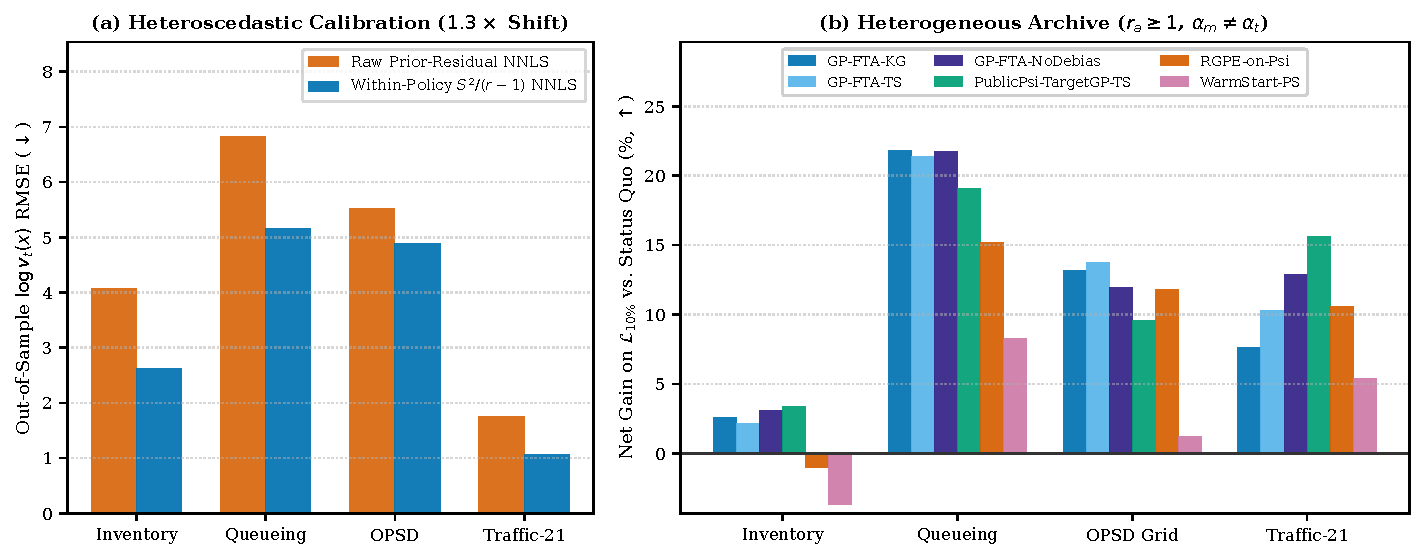
\includegraphics[width=0.98\textwidth]{figures/fig3_diagnostics_and_messy.pdf}
  \caption{(a) Out-of-sample heteroscedastic log-variance RMSE under $1.3\times$ target shift ($r=4$ replications), comparing raw prior-residual NNLS against shift-invariant within-policy $S^2/(r-1)$ NNLS. (b) Mean net gain on $\calL_{10\%}$ relative to status quo across all four operational domains under heterogeneous enterprise source archives ($r_a \ge 1$, $\alpha_m \neq \alpha_t$), including both \texttt{PublicPsi-TargetGP-TS} and \texttt{GP-FTA-NoDebias}.}\label{fig:ec_diagnostics}
\end{figure}

Figure~\ref{fig:ec_diagnostics} and Tables~\ref{tab:messy_archive}--\ref{tab:amortization} report the out-of-sample heteroscedastic calibration diagnostic, the $2{,}108$-run heterogeneous enterprise archive suite (comparing \textbf{GP-FTA-KG}, \textbf{GP-FTA-TS}, \texttt{GP-FTA-NoDebias}, \texttt{PublicPsi-TargetGP-TS}, \texttt{RGPE-on-Psi}, and \texttt{WarmStart-PatternSearch} side by side), the calibrated and stress-test live \texttt{Ingolstadt21} SUMO experiments, and source-archive simulation-call amortization against both raw-policy \texttt{SCBO} and same-representation \texttt{PublicPsi-TargetGP-TS}.

\begin{table}[htbp]
\centering
\caption{Heterogeneous simulated source archives on the shared U3 target panel ($2{,}108$ runs). Logs combine single replications, unequal budgets, incomplete solver coverage, and heterogeneous historical risk tolerances. Two-sided $p$ values compare status-quo loss with frozen GP-FTA-KG and are unadjusted. Online wall time is for $N=60$.}\label{tab:messy_archive}
\scriptsize
\resizebox{\textwidth}{!}{%
\begin{tabular}{llcccccc}
\toprule
\textbf{Family} & \textbf{Method} & \textbf{$N=15$ $\mathcal{L}_{\mathrm{SQ}}$} & \textbf{$N=60$ $\mathcal{L}_{\mathrm{SQ}}$} & \textbf{$N=60$ $\mathcal{L}_{10\%}$} & \textbf{$N=60$ Cert.\%} & \textbf{Two-Sided $p$ ($N=60$)} & \textbf{Online Wall (s)} \\
\midrule
\multirow{9}{*}{Inventory} & \textbf{GP-FTA-KG} & $1.941$ & $1.910$ & $1.910$ & 100.0\% & --- & 41.6 \\
 & \textbf{GP-FTA-TS} & $1.937$ & $1.914$ & $1.920$ & 96.9\% & $0.669$ & 10.0 \\
 & \texttt{GP-FTA-NoDebias} & $1.947$ & $1.901$ & $1.901$ & 100.0\% & $0.632$ & 44.2 \\
 & \texttt{RGPE-on-Psi} & $1.932$ & $1.926$ & $1.983$ & 71.9\% & $0.231$ & 12.4 \\
 & \texttt{WarmStart-PatternSearch} & $1.949$ & $1.943$ & $2.036$ & 53.1\% & $0.016$ & 0.3 \\
 & \texttt{PublicPsi-TargetGP-TS} & $\mathbf{1.909}$ & $\mathbf{1.883}$ & $\mathbf{1.895}$ & 93.8\% & $0.0004$ & 7.9 \\
 & \texttt{RGPE} & $1.963$ & $1.976$ & $1.989$ & 93.8\% & $0.002$ & 72.6 \\
 & \texttt{HyperBO-EB} & $1.974$ & $1.987$ & $1.987$ & 100.0\% & $0.0008$ & 2.1 \\
 & \texttt{STOP} & $1.996$ & $1.996$ & $1.996$ & 100.0\% & $0.003$ & 0.1 \\
\midrule
\multirow{9}{*}{Queueing} & \textbf{GP-FTA-KG} & $2.647$ & $\mathbf{2.518}$ & $\mathbf{2.518}$ & 100.0\% & --- & 44.5 \\
 & \textbf{GP-FTA-TS} & $2.627$ & $2.527$ & $2.527$ & 100.0\% & $0.375$ & 8.8 \\
 & \texttt{GP-FTA-NoDebias} & $\mathbf{2.584}$ & $2.519$ & $2.519$ & 100.0\% & $1.000$ & 44.9 \\
 & \texttt{RGPE-on-Psi} & $2.715$ & $2.688$ & $2.727$ & 87.5\% & $<10^{-4}$ & 10.5 \\
 & \texttt{WarmStart-PatternSearch} & $2.775$ & $2.864$ & $2.955$ & 71.9\% & $<10^{-4}$ & 0.4 \\
 & \texttt{PublicPsi-TargetGP-TS} & $2.704$ & $2.596$ & $2.607$ & 96.9\% & $0.003$ & 6.8 \\
 & \texttt{RGPE} & $3.047$ & $3.012$ & $3.042$ & 90.6\% & $<10^{-4}$ & 53.5 \\
 & \texttt{HyperBO-EB} & $3.056$ & $3.069$ & $3.085$ & 93.8\% & $<10^{-4}$ & 2.8 \\
 & \texttt{STOP} & $2.864$ & $2.864$ & $2.864$ & 100.0\% & $<10^{-4}$ & 0.1 \\
\midrule
\multirow{9}{*}{OPSD Grid} & \textbf{GP-FTA-KG} & $0.0606$ & $0.0568$ & $0.0572$ & 92.9\% & --- & 49.1 \\
 & \textbf{GP-FTA-TS} & $0.0582$ & $0.0566$ & $\mathbf{0.0570}$ & 92.9\% & $0.855$ & 11.1 \\
 & \texttt{GP-FTA-NoDebias} & $0.0589$ & $0.0569$ & $0.0573$ & 92.9\% & $0.903$ & 46.5 \\
 & \texttt{RGPE-on-Psi} & $\mathbf{0.0574}$ & $\mathbf{0.0562}$ & $0.0588$ & 64.3\% & $0.715$ & 13.6 \\
 & \texttt{WarmStart-PatternSearch} & $0.0609$ & $0.0614$ & $0.0635$ & 64.3\% & $0.004$ & 2.0 \\
 & \texttt{PublicPsi-TargetGP-TS} & $0.0607$ & $0.0583$ & $0.0590$ & 85.7\% & $0.358$ & 9.0 \\
 & \texttt{RGPE} & $0.0619$ & $0.0641$ & $0.0643$ & 96.4\% & $0.002$ & 173.9 \\
 & \texttt{HyperBO-EB} & $0.0607$ & $0.0618$ & $0.0626$ & 85.7\% & $0.005$ & 6.1 \\
 & \texttt{STOP} & $0.0639$ & $0.0639$ & $0.0639$ & 100.0\% & $0.0009$ & 0.4 \\
\midrule
\multirow{9}{*}{Traffic-21} & \textbf{GP-FTA-KG} & $1.102$ & $1.082$ & $1.110$ & 78.1\% & --- & 76.4 \\
 & \textbf{GP-FTA-TS} & $1.088$ & $1.061$ & $1.078$ & 87.5\% & $0.135$ & 37.4 \\
 & \texttt{GP-FTA-NoDebias} & $1.088$ & $1.034$ & $1.043$ & 93.8\% & $0.003$ & 78.2 \\
 & \texttt{RGPE-on-Psi} & $1.090$ & $1.055$ & $1.072$ & 87.5\% & $0.252$ & 45.3 \\
 & \texttt{WarmStart-PatternSearch} & $1.106$ & $1.096$ & $1.135$ & 68.8\% & $0.241$ & 2.1 \\
 & \texttt{PublicPsi-TargetGP-TS} & $\mathbf{1.050}$ & $\mathbf{1.007}$ & $\mathbf{1.007}$ & 100.0\% & $0.001$ & 34.3 \\
 & \texttt{RGPE} & $1.112$ & $1.094$ & $1.126$ & 75.0\% & $0.188$ & 13.1 \\
 & \texttt{HyperBO-EB} & $1.138$ & $1.137$ & $1.202$ & 46.9\% & $0.005$ & 2.7 \\
 & \texttt{STOP} & $1.088$ & $1.088$ & $1.113$ & 81.2\% & $0.524$ & 0.4 \\
\bottomrule
\end{tabular}%
}
\end{table}
\begin{table}[htbp]
\centering
\caption{Microscopic \texttt{Ingolstadt21} SUMO evaluation ($N=15$). The calibrated U3 panel has eight threshold and weight configurations of one network and route, with two simulation streams per configuration. The 40 uncalibrated stress runs were retained from the earlier experiment.}\label{tab:live_sumo}
\scriptsize
\setlength{\tabcolsep}{4.6pt}
\begin{tabular}{llccccc}
\toprule
\textbf{Regime} & \textbf{Method} & \textbf{Status-Quo Loss} & \textbf{Challenger $J_t^{\ddagger}$} & \textbf{Cert./runs} & \textbf{S/A/U$^*$} & \textbf{Actual Calls} \\
\midrule
\multirow{9}{*}{Calibrated ($144$ runs)} & \textbf{GP-FTA-KG} & $\mathbf{0.9439} \pm 0.0181$ & $0.9340$ & 8/16 & 3/5/0 & 344.8 \\
 & \texttt{PublicPsi-TargetGP-TS} & $0.9696 \pm 0.0088$ & $0.9661$ & 5/16 & 3/2/0 & 387.8 \\
 & \textbf{GP-FTA-TS} & $0.9737 \pm 0.0090$ & $0.9647$ & 5/16 & 1/4/0 & 362.2 \\
 & \texttt{SCBO-on-Psi} & $0.9829 \pm 0.0050$ & $0.9735$ & 3/16 & 2/1/0 & 379.8 \\
 & \texttt{RGPE-on-Psi} & $0.9850 \pm 0.0058$ & $1.0247$ & 2/16 & 0/2/0 & 396.5 \\
 & \texttt{WarmStart-PatternSearch} & $0.9871 \pm 0.0037$ & $0.9898$ & 3/16 & 1/2/0 & 379.8 \\
 & \texttt{RGPE} & $0.9941 \pm 0.0012$ & $1.0164$ & 0/16 & --- & 422.0 \\
 & \texttt{SCBO} & $0.9941 \pm 0.0012$ & $0.9909$ & 0/16 & --- & 422.0 \\
 & \texttt{STOP} & $0.9941 \pm 0.0012$ & $0.9878$ & 0/16 & --- & 392.0 \\
\midrule
\multirow{5}{*}{Stress Test ($40$ runs)} & \texttt{TLS-OLH-KG} (Legacy) & $0.9876$ & $0.9642$ & 0/8 & --- & 422.0 \\
 & \texttt{SCBO} & $0.9876$ & $0.9826$ & 0/8 & --- & 422.0 \\
 & \texttt{RGPE} & $0.9876$ & $0.9888$ & 0/8 & --- & 422.0 \\
 & \texttt{Target-SPSA} & $0.9876$ & $0.9645$ & 0/8 & --- & 422.0 \\
 & \texttt{STOP} & $0.9876$ & $0.9876$ & 0/8 & --- & 392.0 \\
\bottomrule
\end{tabular}
\par\smallskip\parbox{\textwidth}{\scriptsize $^*$S/A/U counts certified deployments classified as confidently safe, boundary-ambiguous, or confidently unsafe by an independent audit. A dash indicates no audited deployment. $^{\ddagger}$Calibrated runs use the frozen primary. Stress runs use the saved uncertified candidate.}
\end{table}
\begin{table}[htbp]
\centering
\caption{Source-archive simulation-call amortization ($B_{\mathrm{src}}=1{,}428$ calls per family) comparing low-budget \textbf{GP-FTA-KG} ($N=15$) against both raw-policy \texttt{SCBO} ($N=60$) and same-representation \texttt{PublicPsi-TargetGP-TS} ($N=60$). Full-cost break-even $M_{\mathrm{break}}^{\mathrm{full}}$ is reported only when \textbf{GP-FTA-KG} ($N=15$) attains equal or lower mean $\mathcal{L}_{\mathrm{SQ}}$ than the $N=60$ cold-start comparator (`Not dom.' indicates the $N=60$ cold-start representation control achieves lower loss).}\label{tab:amortization}
\scriptsize
\resizebox{\textwidth}{!}{%
\begin{tabular}{llcccccc}
\toprule
\textbf{Comparator ($N=60$)} & \textbf{Family} & \textbf{GP-FTA ($N\!=\!15$)} & \textbf{Cold ($N\!=\!60$)} & \textbf{$B_{\mathrm{FTA},15}$ / $B_{\mathrm{cold},60}$} & \textbf{Call Saving $\Delta B$ [95\% CI]} & \textbf{$M_{\mathrm{break}}^{\mathrm{sunk}}$} & \textbf{$M_{\mathrm{break}}^{\mathrm{full}}$ (95\% UB)} \\
\midrule
\multirow{4}{*}{\texttt{SCBO}} & Inventory & $1.927$ & $1.960$ & 238.8 / 350.2 & $+111.5$ $[+54.2, +168.8]$ & $1$ & $\mathbf{13}$ ($\le 27$) \\
 & Queueing & $2.535$ & $3.052$ & 254.4 / 312.4 & $+58.0$ $[+16.0, +100.0]$ & $1$ & $\mathbf{25}$ ($\le 90$) \\
 & OPSD Grid & $0.0587$ & $0.0610$ & 260.3 / 406.4 & $+146.1$ $[+106.2, +186.1]$ & $1$ & $\mathbf{10}$ ($\le 14$) \\
 & Traffic-21 & $1.108$ & $1.145$ & 285.4 / 426.8 & $+141.4$ $[+103.2, +179.5]$ & $1$ & $\mathbf{11}$ ($\le 14$) \\
\midrule
\multirow{4}{*}{\texttt{PublicPsi-TargetGP-TS}} & Inventory & $1.927$ & $1.883$ & 238.8 / 390.2 & $+151.5$ $[+111.4, +191.6]$ & Not dom. & Not dom. \\
 & Queueing & $2.535$ & $2.596$ & 254.4 / 385.1 & $+130.8$ $[+97.0, +164.5]$ & $1$ & $\mathbf{11}$ ($\le 15$) \\
 & OPSD Grid & $0.0587$ & $0.0583$ & 260.3 / 416.0 & $+155.7$ $[+121.8, +189.7]$ & Not dom. & Not dom. \\
 & Traffic-21 & $1.108$ & $1.007$ & 285.4 / 372.4 & $+87.0$ $[+40.0, +134.0]$ & Not dom. & Not dom. \\
\bottomrule
\end{tabular}%
}
\end{table}



\end{document}
